%! Author = Len Washington III
%! Date = 3/2/24

% Preamble
\documentclass[title={Chapter 9}]{fdsn201notes}

% Packages

% Document
\begin{document}%
%
\maketitle{9}%
%
\begin{table}[H]
	\centering
	\begin{threeparttable}
		\caption{Nutrients for Healthy Tissues}
		\label{tab:healthy-nutrient-tissues}
		\rowcolors{2}{rowmedgreen}{rowlightgreen}
		\begin{tabular}{p{0.4\textwidth} p{0.6\textwidth}}
			\rowcolor{rowdarkgreen}\textbf{Nutrient} & \textbf{Recommended Intake}\\
			Iron & RDA for 19 to 50 years of age:

			Women 18 mg/day

			Men = 8 mg/day\\
			Zinc & RDA for 19 to 50 years of age:

			Women = 8 mg/day

			Men = 11 mg/day\\
			Copper & RDA for 19 to 50 years of age: 90 $\mu$g/day\\
			Vitamin B6 (pyridoxine) & RDA for 19 to 50 years of age: 1.3 mg/day

			RDA for 51 years of age and older:

			Women 1.5 mg/day

			Men 1.7 mg/day \\
			Folate (folic acid) & RDA for 19 years of age and older:

			400 $\mu$g/day \\
			Vitamin B12 (cobalamin) & RDA for 19 years of age and older:

			2.4 $\mu$g/day\\
			Vitamin K & Al for 19 to 50 years of age:

			Women = 90 $\mu$g/day

			Men 120 $\mu$g/day\\
			Vitamin C & RDA for 19 years of age and older.

			Women 75 mg/day

			Men 90 mg/day

			Smokers = 35 mg more per day than RDA\\
			Calcium & RDA for 19 to 50 years of age: 1,000 mg/day

			Women 51 years of age and older = 1,200 mg/day

			Men 51 to 70 years of age = 1,000 mg/day; 70 years of age and older = 1,200 mg/day\\
			Phosphorus & RDA for 19 years of age and older.

			700 mg/day\\
			Magnesium & RDA for 19 to 30 years of age:

			Women = 310 mg/day

			Men = 400 mg/day

			RDA for 31 years of age and older:

			Women = 320 mg/day

			Men = 420 mg/day\\
			Fluoride & RDA for 19 years of age and older:

			Women = 3 mg/day

			Men = 4 mg/day\\
			Vitamin D & RDA for 19 to 70 years of age:$^{*}$ 600 IU/day

			RDA for 71 years of age and older: 800 IU/day\\
			\rowcolor{rowdarkgreen} & \\
		\end{tabular}
		\begin{tablenotes}
			\small
			\item To see the full profile of all micronutrients, turn to the In Depth essay following Chapter 6, Vitamins and Minerals: Micronutrients with Macro Powers (pages 211--221).

			$^{*}$Based on the assumption that a person does not get adequate sun exposure.
		\end{tablenotes}
	\end{threeparttable}
\end{table}

\section{Components of the Blood}\label{sec:Components of the Blood}
\begin{itemize}
	\item \definition{Erythrocytes}{red blood cells}
	\item \definition{Leukocytes}{white blood cells; key to our immune function}
	\item \definition{Platelets}{cell fragments that assist in the formation of blood clots}
	\item \definition{Plasma}{the watery matrix of blood in which the cells and platelets flow}
\end{itemize}

\begin{figure}[H]
	\centering
	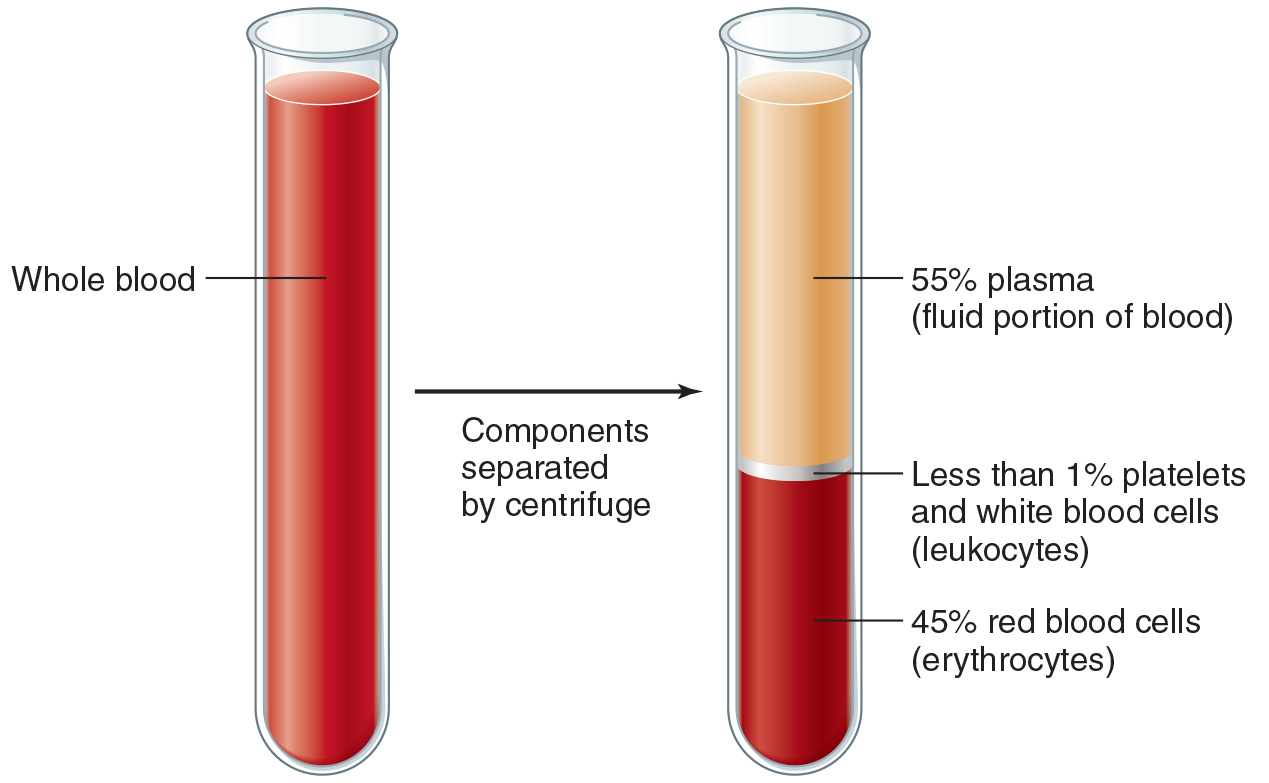
\includegraphics[width=\textwidth]{9_components_of_the_blood}
	\caption{Components of the Blood}
	\label{fig:components-of-the-blood}
\end{figure}


\section{Iron}\label{sec:Iron}
\begin{itemize}
	\item Iron is a component of numerous proteins in the body
	\begin{itemize}
		\item Approximately two-thirds of the body’s iron is found in the hemoglobin, the oxygen-carrying protein, of the red blood cells
		\item Iron can also be found in myoglobin, which is similar to hemoglobin but is found in the muscle cells
	\end{itemize}
\end{itemize}

\begin{figure}[H]
	\centering
	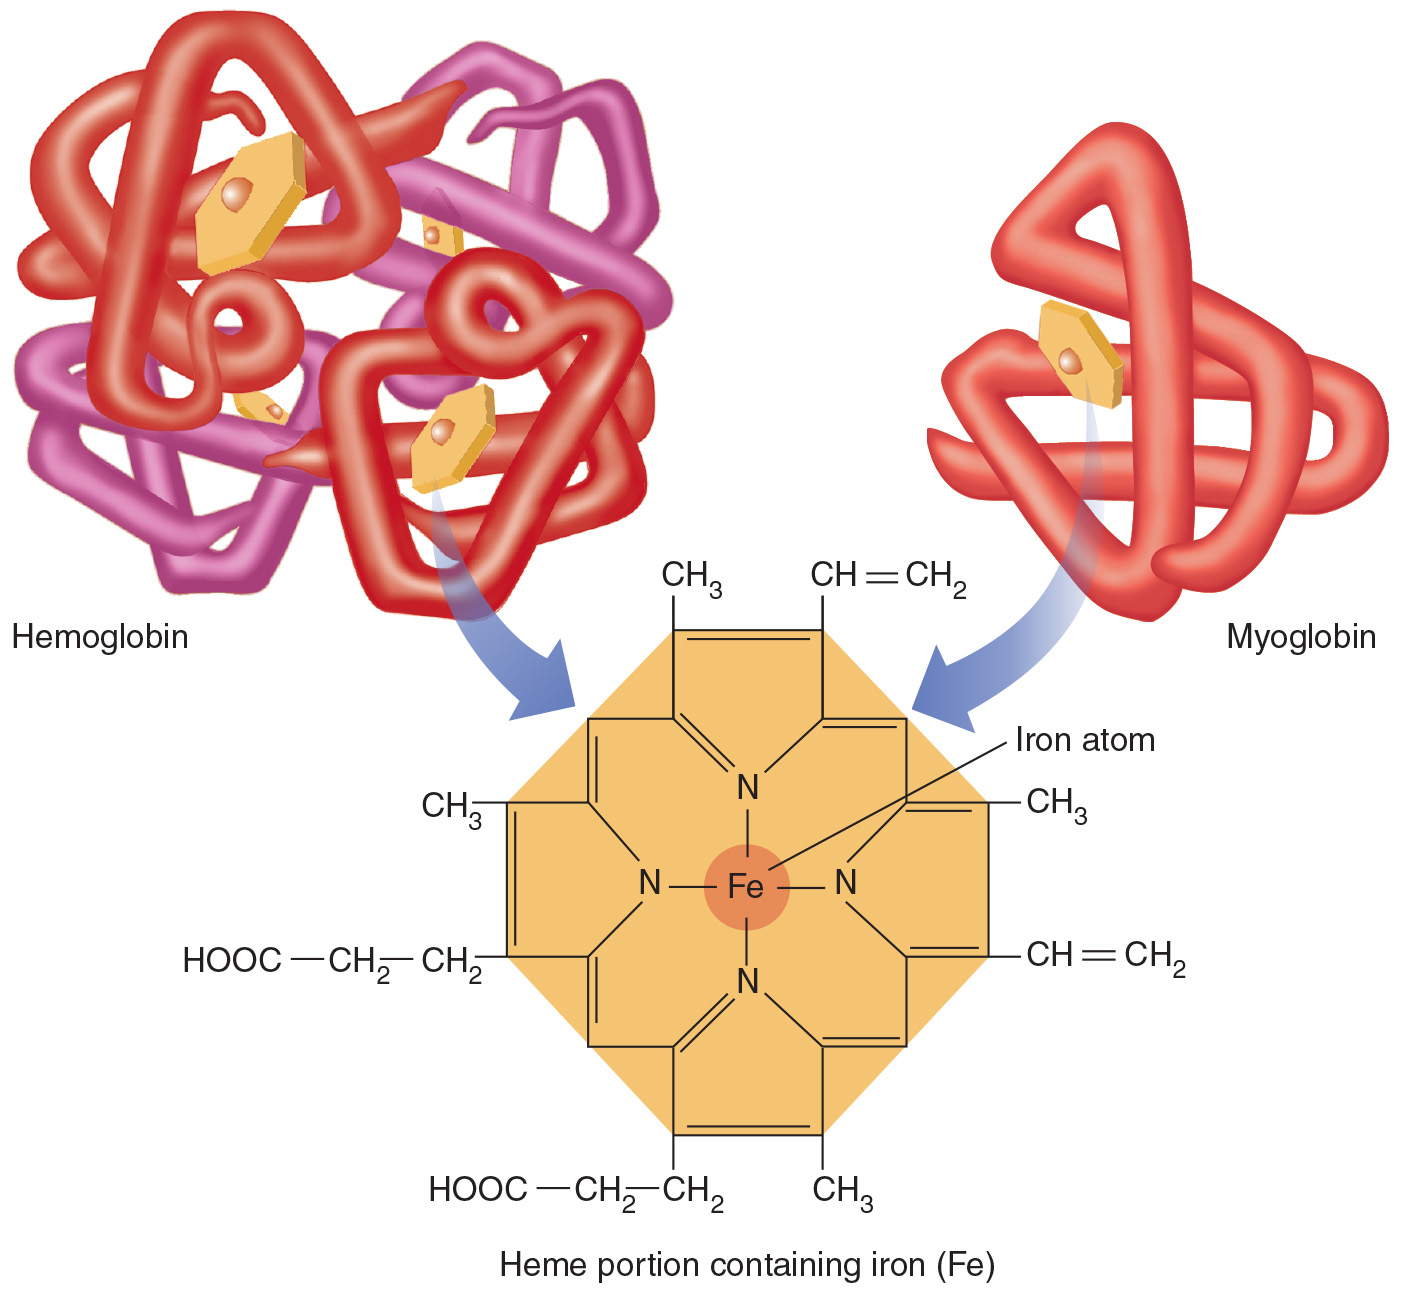
\includegraphics[width=\textwidth]{9_iron}
	\caption{Iron}
	\label{fig:iron}
\end{figure}

\section{Iron Storage and Recycling}\label{sec:iron-storage-and-recycling}
\begin{itemize}
	\item Extra iron can be stored in the liver, intestinal mucosa, bone marrow, and spleen
	\item As red blood cells break down their iron is released and can be recycled
	\begin{itemize}
		\item The liver and spleen are responsible for iron-recycling, which decreases our need for dietary iron
	\end{itemize}
\end{itemize}

\section{Iron Absorption}\label{sec:iron-absorption}
\begin{itemize}
	\item The body’s ability to absorb iron are influenced by:
	\begin{itemize}
		\item Iron status
		\item Stomach acid
		\item Iron content in the diet
		\item Type of iron consumed
		\item Other dietary factors; phytates, polyphenols, and other minerals
	\end{itemize}
\end{itemize}

\begin{table}[H]
	\centering
	\begin{threeparttable}
		\caption{Circumstances Affecting Iron Status}
		\label{tab:circumstances-affecting-iron-status}
		\rowcolors{2}{rowmedgreen}{rowlightgreen}
		\begin{tabular}{p{0.5\textwidth} p{0.5\textwidth}}
			\rowcolor{rowdarkgreen}\textbf{Circumstances That Improve Iron Status} & \textbf{Circumstances That Diminish Iron Status}\\
			\begin{itemize}
				\item Use of oral contraceptives-reduces menstrual blood loss in women.
				\item Breastfeeding-delays resumption of menstruation in new mothers and thereby reduces menstrual blood loss. It is therefore an important health measure, especially in developing nations.
				\item Consumption of iron-containing foods and supplements.
			\end{itemize}
			& \begin{itemize}
				\item Use of hormone replacement therapy--can cause uterine bleeding.
				\item Eating a vegetarian diet--reduces or eliminates sources of heme iron.
				\item Intestinal parasitic infection--causes intestinal bleeding. Iron-deficiency anemia is common in people with intestinal parasitic infection.
				\item Blood donation--reduces iron stores; people who donate frequently,
				  particularly premenopausal women, may require iron supplementation.
				\item Intense endurance exercise training--appears to increase risk for inflammation, suboptimal iron intake, increased iron loss due to rupture of red blood cells, and losses in sweat and feces.
			\end{itemize}\\
			\rowcolor{rowdarkgreen} & \\
		\end{tabular}
		\begin{tablenotes}
			\small
			\item Source: Data from Dietary Reference Intakes for Vitamin A, Vitamin K, Arsenic, Boron, Chromium, Copper, Iodine, Manganese, Molybdenum, Nickel, Silicon, Vanadium, and Zinc © 2002 by the National Academy of Sciences, National Academies Press.
		\end{tablenotes}
	\end{threeparttable}
\end{table}

\begin{figure}[H]
	\centering
	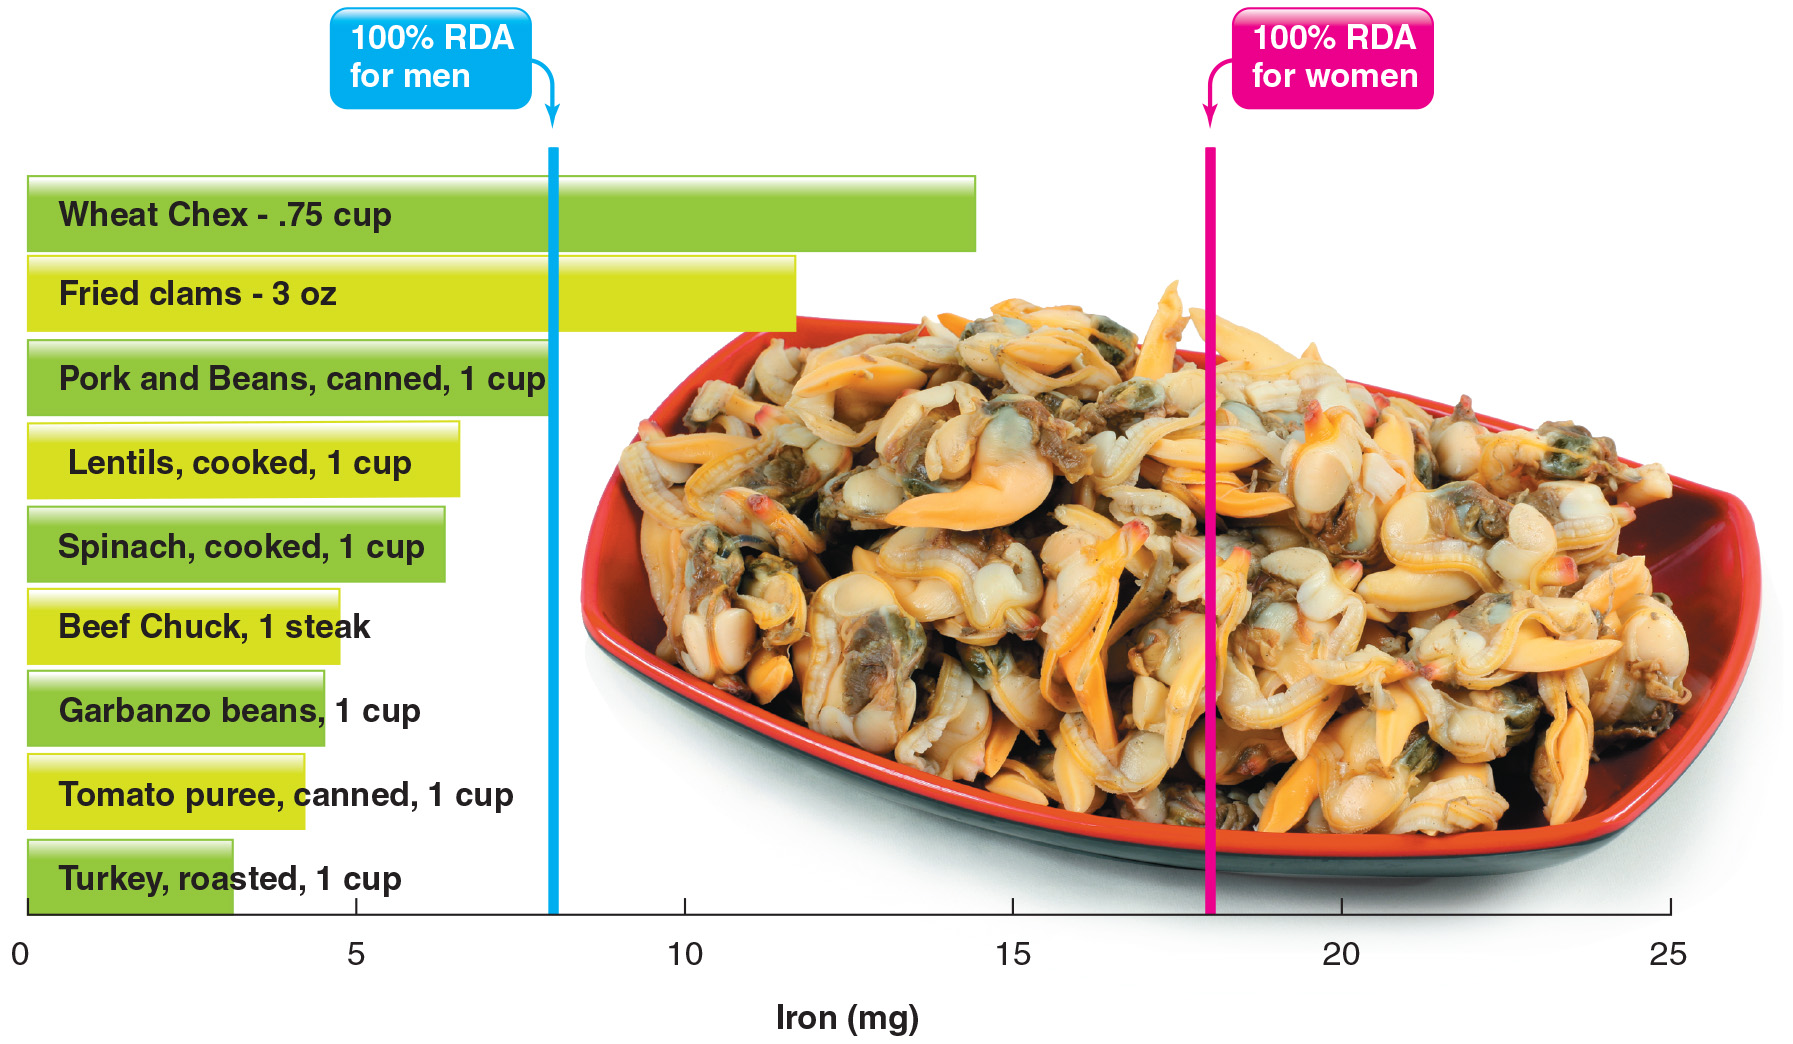
\includegraphics[width=\textwidth]{9_common_sources_iron}
	\caption{Common Food Sources of Iron}
	\label{fig:common-food-sources-of-iron}
\end{figure}

\begin{itemize}
	\item Iron toxicity
	\begin{itemize}
		\item In the U.S.\ accidental ion overdose is the leading cause of death in children under 6
		\item Can cause nausea and constipation in mild cases
	\end{itemize}
	\item Iron deficiency
	\begin{itemize}
		\item Iron deficiency anemia causes the red blood cells to be smaller and paler than normal
	\end{itemize}
\end{itemize}

\section{Zinc}\label{sec:Zinc}
\begin{itemize}
	\item Functions of zinc include
	\begin{itemize}
		\item Enzymatic functions--over 300 enzymes in the human body use zinc
		\item Structural functions--helps to stabilize proteins so that they function properly
		\item Regulatory functions--helps to regulate gene expression
	\end{itemize}
	Only 10--35\% of dietary zinc is absorbed
	Factors decreasing absorption include:
	\begin{itemize}
		\item Non-heme iron intake
		\item Phytates
		\item Fiber
	\end{itemize}
	\item Toxicity is rare, but is mainly seen with over consumption of zinc supplements
	\item Deficiency is rare in the U.S. but can be seen in other countries where diets are predominantly bread or grain based
	\begin{itemize}
		\item Symptoms include growth retardation, delayed sexual maturation, and increased risk of infections
	\end{itemize}
\end{itemize}

\section{Copper}\label{sec:Copper}
\begin{itemize}
	\item Trace mineral that is crucial for blood health
	\item Component of ceruloplasmin
	\begin{itemize}
		\item Protein used in iron transport
	\end{itemize}
	\item Energy metabolism
	\item Building of connective tissues
	\item Toxicity is not well studied in humans
	\item Deficiencies are rare but can lead to
	\begin{itemize}
		\item Inhibition of hemoglobin synthesis
		\item Inadequate iron utilization
		\item Microcytic anemia
	\end{itemize}
\end{itemize}

\begin{figure}[H]
	\centering
	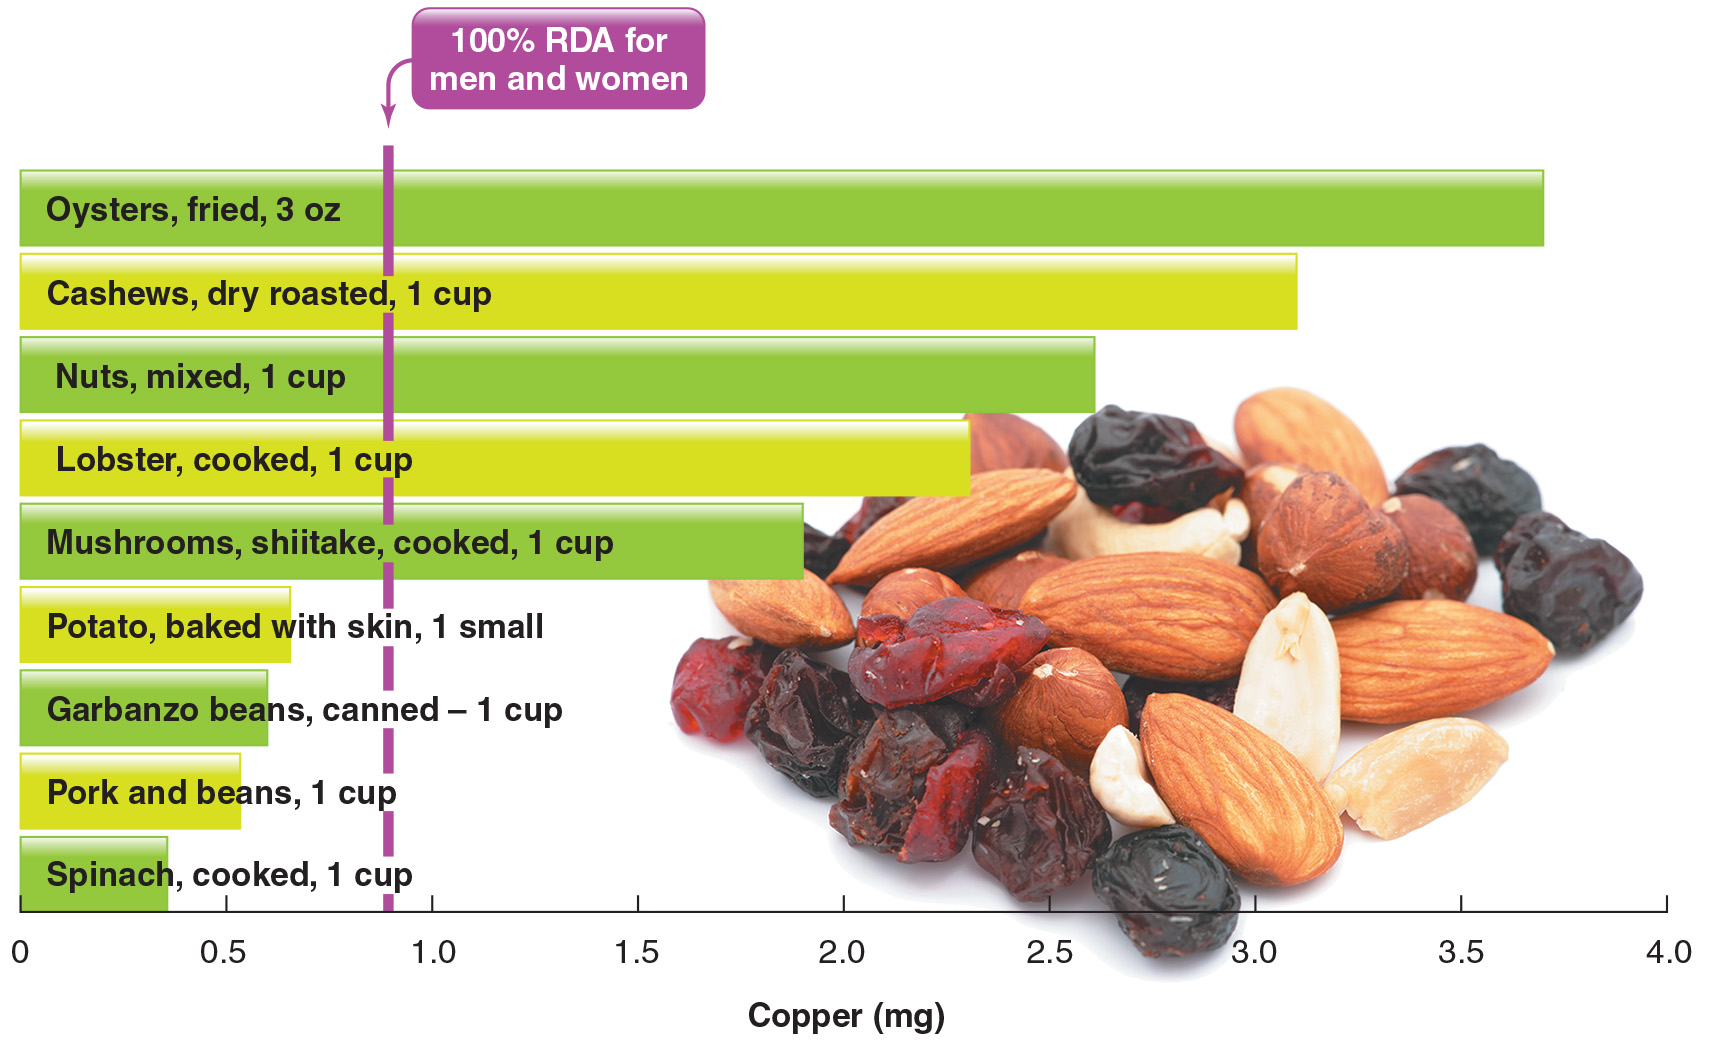
\includegraphics[width=\textwidth]{9_copper}
	\caption{Copper}
	\label{fig:copper}
\end{figure}

\begin{figure}[H]
	\centering
	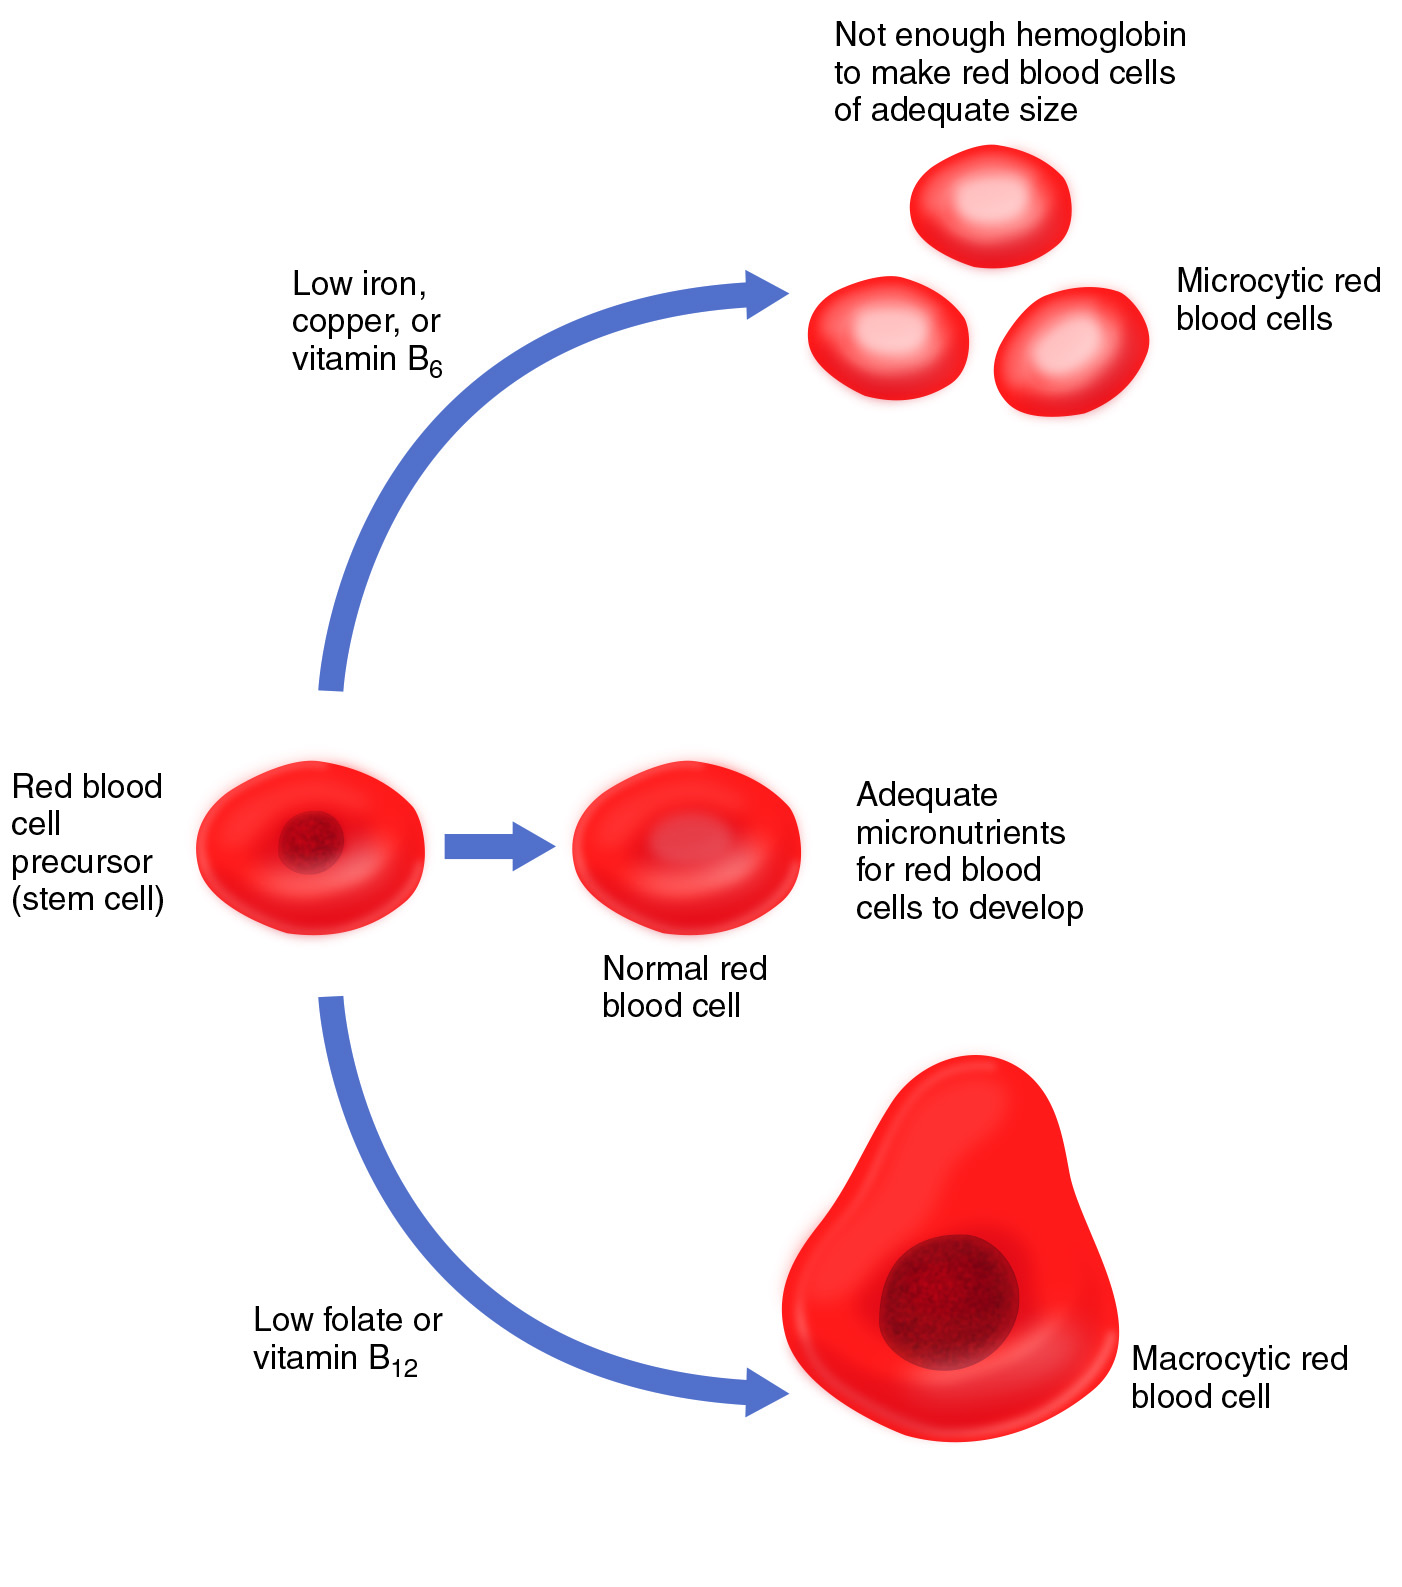
\includegraphics[width=\textwidth]{9_vitamin_roles_in_blood_formation}
	\caption{Vitamin Roles in Blood Formation}
	\label{fig:vitamin-roles-in-blood-formation}
\end{figure}

\section{Vitamin K}\label{sec:vitamin-k}
\begin{itemize}
	\item Fat-soluble vitamin
	\item Stored primarily in the liver
	\item Phylloquinone: plant form of vitamin K
	\item Menaquinone: form of vitamin K produced by bacteria in the large intestine
	\item Functions of vitamin K
	\begin{itemize}
		\item Blood clotting (prothrombin synthesis)
		\item Bone metabolism (osteocalcin synthesis)
	\end{itemize}
	\item Recommended intake
	\begin{itemize}
		\item There is no RDA for vitamin K
		\item AI values are 120 $\mu$g/day for men and 90 $\mu$g/day for women
	\end{itemize}
	\item Sources of vitamin K
	\begin{itemize}
		\item Green leafy vegetables, vegetable oils
	\end{itemize}
	\item What if you consume too much vitamin K?
	\begin{itemize}
		\item No side effects from large quantities
	\end{itemize}
	\item What if you don’t consume enough vitamin K?
	\begin{itemize}
		\item Reduced blood clotting, excessive bleeding
		\item Occurs with diseases that limit absorption of fat in the small intestine
	\end{itemize}
\end{itemize}

\section{Vitamin C}\label{sec:vitamin-c-9}
\begin{itemize}
	\item Vitamin C helps to produce and maintain healthy collagen
	\begin{itemize}
		\item Collagen is a fibrous protein found in the bone, teeth, tendons, blood vessels, and gum tissue
	\end{itemize}
	\item Assists in the synthesis of
	\begin{itemize}
		\item DNA
		\item Bile
		\item Serotonine
		\item Carnitine
	\end{itemize}
	\item Recommended intake
	\begin{itemize}
		\item 90 mg/day for men; 75 mg/day for women
		\item Smokers need an extra 35 mg/day
		\item UL is 2,000 mg/day for adults
	\end{itemize}
	\item Sources of vitamin C
	\begin{itemize}
		\item Fresh fruits and vegetables
		\item Heat destroys vitamin C
		\item Cooking foods lowers their vitamin C content
	\end{itemize}
\end{itemize}

\begin{figure}[H]
	\centering
	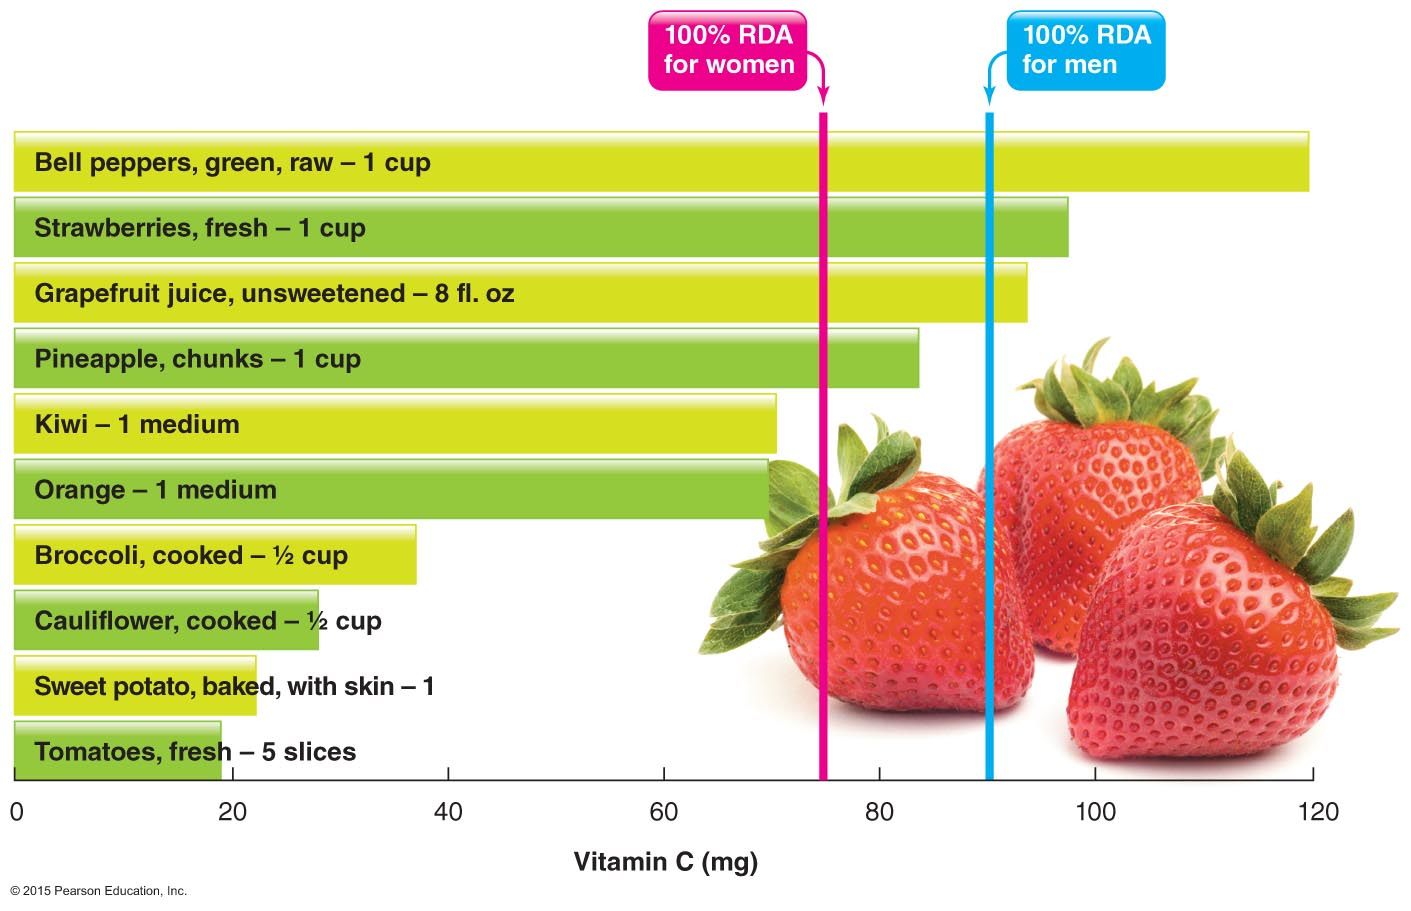
\includegraphics[width=\textwidth]{9_common_sources_vitamin_c}
	\caption{Common Food Sources of Vitamin C}
	\label{fig:common-sources-vitamin-c}
\end{figure}

\begin{itemize}
	\item What if you consume too much vitamin C?
	\begin{itemize}
		\item Megadoses (ten times or more of the recommended intake) of vitamin C can cause nausea, diarrhea, nosebleeds, and abdominal cramps
		\item Can cause iron toxicity in people with hemochromatosis
		\item Can lead to kidney stone formation in people with kidney disease
	\end{itemize}
	\item What if you don’t consume enough vitamin C?
	\begin{itemize}
		\item Scurvy is the most common vitamin C deficiency disease
		\begin{itemize}
			\item Bleeding gums, loose teeth, wounds that fail to heal, swollen ankles and wrists, bone pain and fractures, diarrhea, weakness, and depression
		\end{itemize}
		\item Anemia can also result from vitamin C deficiency
	\end{itemize}
\end{itemize}

\begin{figure}[H]
	\centering
	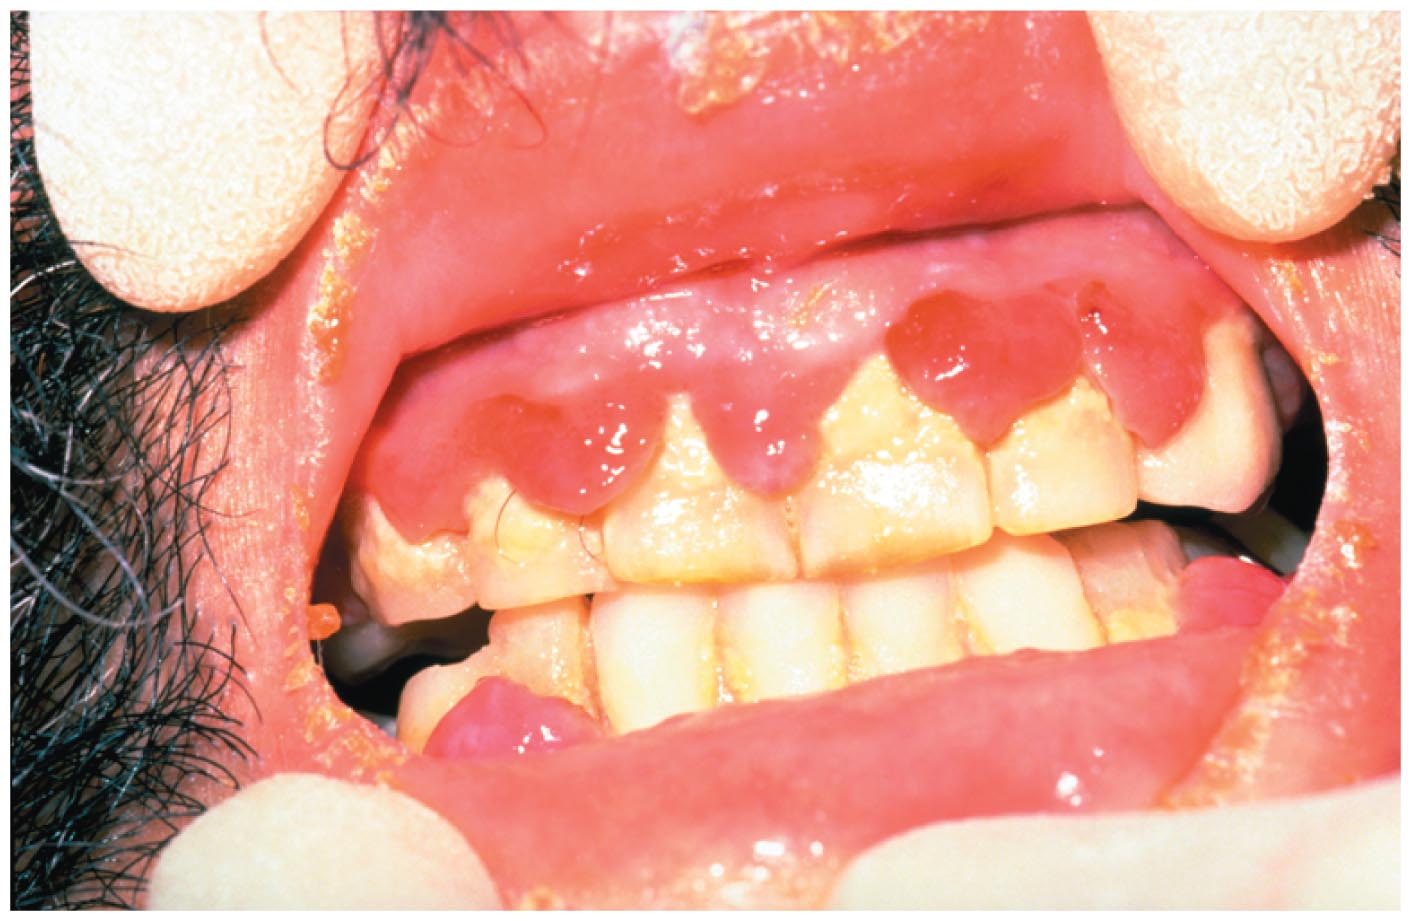
\includegraphics[width=\textwidth]{8_scurvy}
	\caption{Scurvy}
	\label{fig:9_scurvy}
\end{figure}

\section{Bone Health}\label{sec:bone-health}
\begin{itemize}
	\item Bone structure
	\begin{itemize}
		\item Provides strength to support the body
		\item Allows for flexibility
		\item Contains about 65\% minerals, providing the hardness of bone
		\item Contains 35\% organic structures for strength, durability, and flexibility
		\item \definition{Collagen}{fibrous protein in bone tissue}
	\end{itemize}
\end{itemize}

\begin{table}[H]
	\centering
	\caption{Functions of Bone in the Human Body}
	\label{tab:functions-of-bone}
	\rowcolors{2}{rowmedgreen}{rowlightgreen}
	\begin{tabular}{p{0.5\textwidth}p{0.5\textwidth}}
		\rowcolor{rowdarkgreen}\textbf{Functions Related to Structure and Support} & \textbf{Functions Related to Metabolic Processes}\\
		\begin{itemize}
			\item Bones provide physical support for organs and body segments.
			\item Bones protect vital organs; for example, the rib cage protects the lungs, the skull protects the brain, and the vertebrae of the spine protect the spinal cord.
			\item Bones work with muscles and tendons to allow movement-muscles attach to bones via tendons, and their contraction produces movement at the body's joints.
		\end{itemize} & \begin{itemize}
			\item Bone tissue acts as a storage reservoir for many minerals, including calcium, phosphorus, and fluoride. The body draws upon such deposits when these minerals are needed for various body processes; however, this can reduce bone mass.
			\item Most blood cells are produced in the bone marrow.
		\end{itemize}\\
		\rowcolor{rowdarkgreen} & \\
	\end{tabular}
\end{table}

\begin{itemize}
	\item Two types of bone tissue
	\begin{itemize}
		\item \definition{Cortical bone (compact bone)}{very dense tissue making up 80\% of the skeleton}
		\begin{itemize}
			\item Outer surface of all bones
			\item Many of the small bones (wrists, hands, feet)
		\end{itemize}
		\item \definition{Trabecular bone (spongy bone)}{``scaffolding'' on the inside of bones; supports cortical bone and makes up 20\% of the skeleton}
		\begin{itemize}
			\item Faster turnover rate
		\end{itemize}
	\end{itemize}
\end{itemize}

\begin{figure}[H]
	\centering
	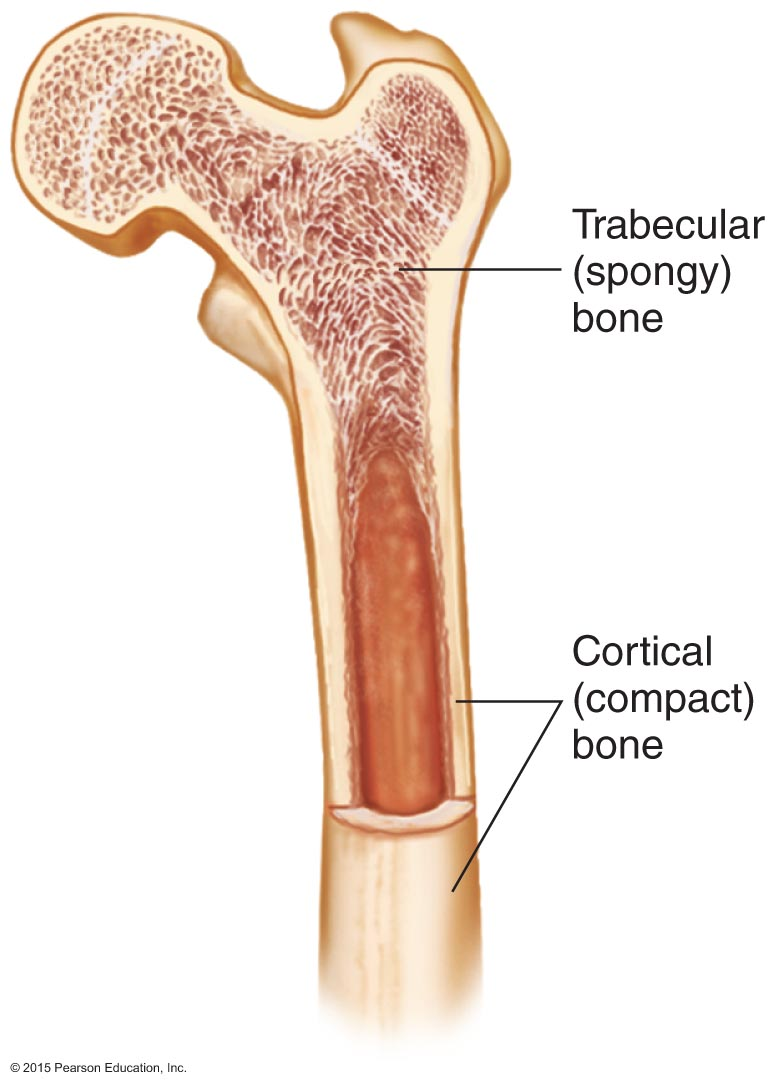
\includegraphics[height=0.5\paperheight]{9_bone_structure}
	\caption{Bone Structure}
	\label{fig:bone-structure}
\end{figure}

\begin{itemize}
	\item Bones develop through three processes
	\begin{itemize}
		\item Bone growth--increase in bone size
		\item Bone modeling--shaping of bone
		\begin{itemize}
			\item Size and shape do not change significantly after puberty
			\item Bone density--degree of compactness of bone tissue; continues to develop into early adulthood
		\end{itemize}
		\item Bone remodeling--reshaping of bone; occurs throughout life
		\begin{itemize}
			\item Bone remodeling involves
			\begin{itemize}
				\item \definition{Resorption}{surface of bones is broken down}
				\item \definition{Osteoclasts}{cells that erode the surface of bones}
				\item Formation of new bone by cells called osteoblasts
				\item Osteoblasts produce the collagen-containing component of bone
			\end{itemize}
		\end{itemize}
	\end{itemize}
\end{itemize}

\begin{figure}[H]
	\centering
	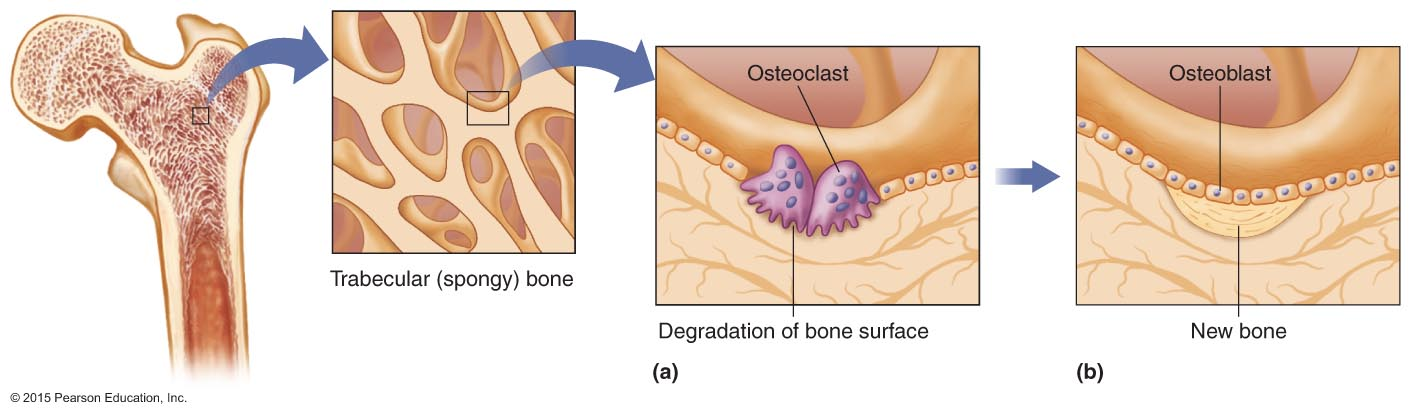
\includegraphics[width=\textwidth]{9_bone_remodeling}
	\caption{Bone Remodeling}
	\label{fig:bone-remodeling}
\end{figure}

\section{Assessing Bone Health}\label{sec:assessing-bone-health}
\begin{itemize}
	\item Dual-energy x-ray absorptiometry (DXA or DEXA)
	\begin{itemize}
		\item Measures bone density
		\item Uses very-low-level x-ray energy
		\item Provides a full body scan or can be used to scan peripheral regions (wrist, heel)
		\item Is a noninvasive procedure
		\item Recommended for postmenopausal women
		\item A T-score is obtained, which compares bone density to that of a healthy 30-year-old
	\end{itemize}
\end{itemize}

\begin{figure}[H]
	\centering
	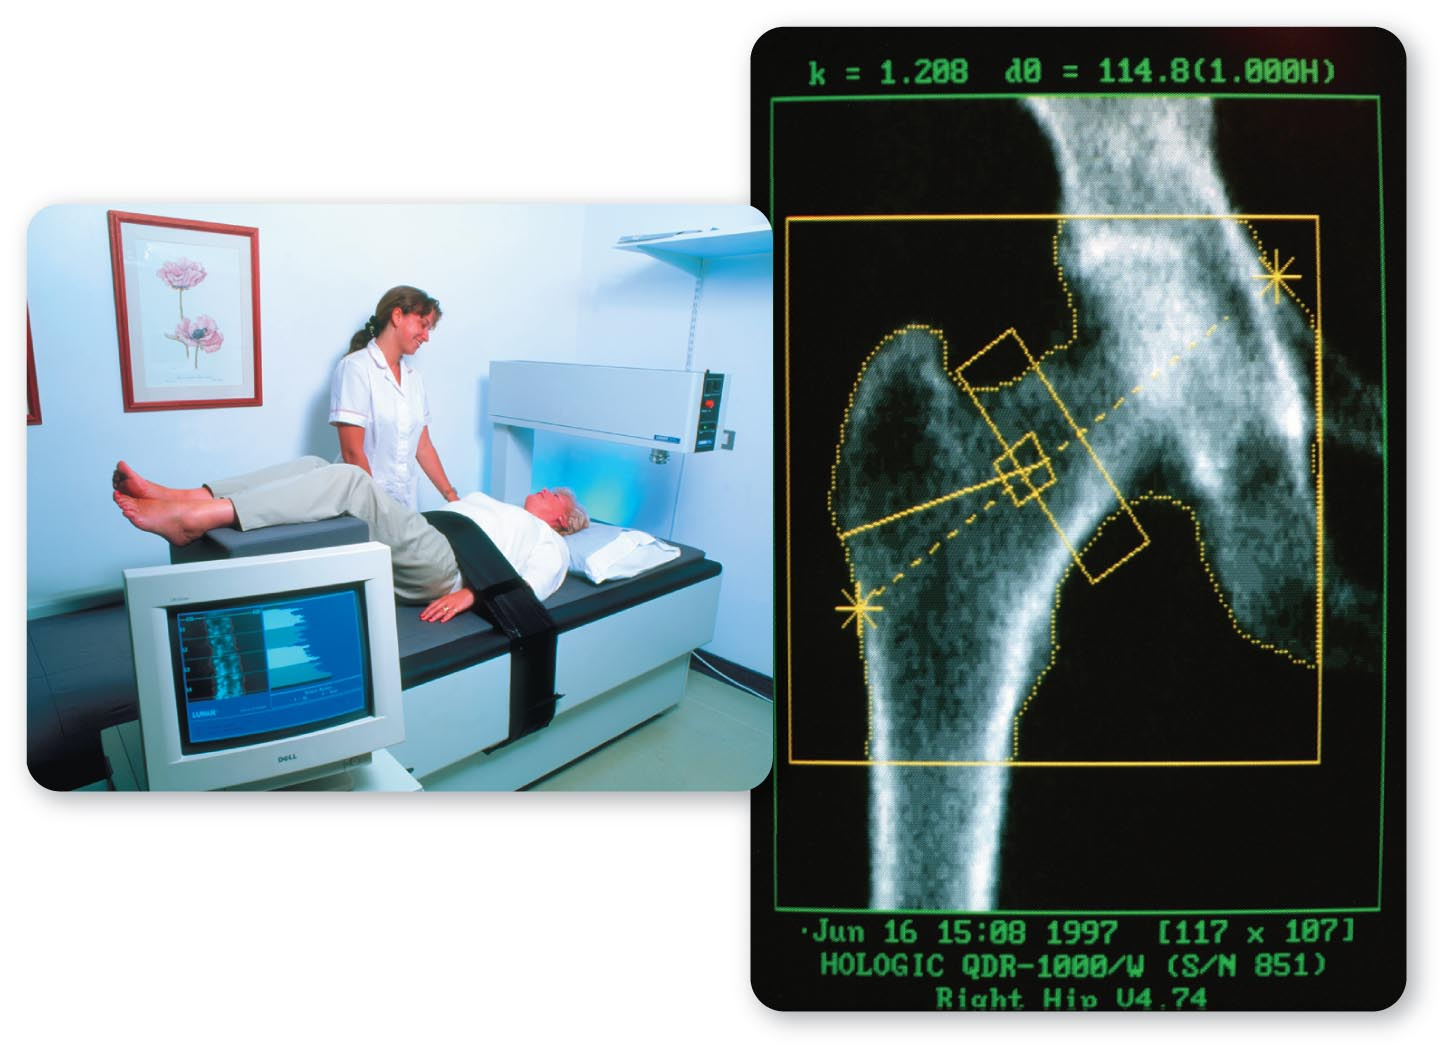
\includegraphics[width=\textwidth]{9_dxa}
	\caption{DXA}
	\label{fig:dxa}
\end{figure}

\section{Calcium}\label{sec:calcium}
\begin{itemize}
	\item The most abundant major mineral in the body
	\begin{itemize}
		\item 99\% of body calcium is found in bone
		\item 1\% is found in blood and soft tissues
	\end{itemize}
	\item Functions of calcium
	\begin{itemize}
		\item Forms and maintains bones and teeth
		\item Assists with acid--base balance
		\item Critical for normal transmission of nerve impulses
		\item Assists in muscle contraction
	\end{itemize}
	\item Blood calcium level is tightly controlled
	\item Low calcium level
	\begin{itemize}
		\item Parathyroid hormone (PTH) is released
		\item PTH stimulates activation of vitamin D
		\item PTH and vitamin D cause
		\begin{itemize}
			\item Kidneys to retain more calcium
			\item Osteoclasts to break down bone and release calcium
			\item Stimulation of calcium absorption from intestines
		\end{itemize}
	\end{itemize}
	\item High calcium level
	\begin{itemize}
		\item Thyroid gland releases calcitonin
		\item Calcitonin functions to
		\begin{itemize}
			\item Prevent calcium reabsorption from kidneys
			\item Limit calcium absorption from intestines
			\item Inhibit osteoclasts from breaking down bone
		\end{itemize}
	\end{itemize}
\end{itemize}

\begin{figure}[H]
	\centering
	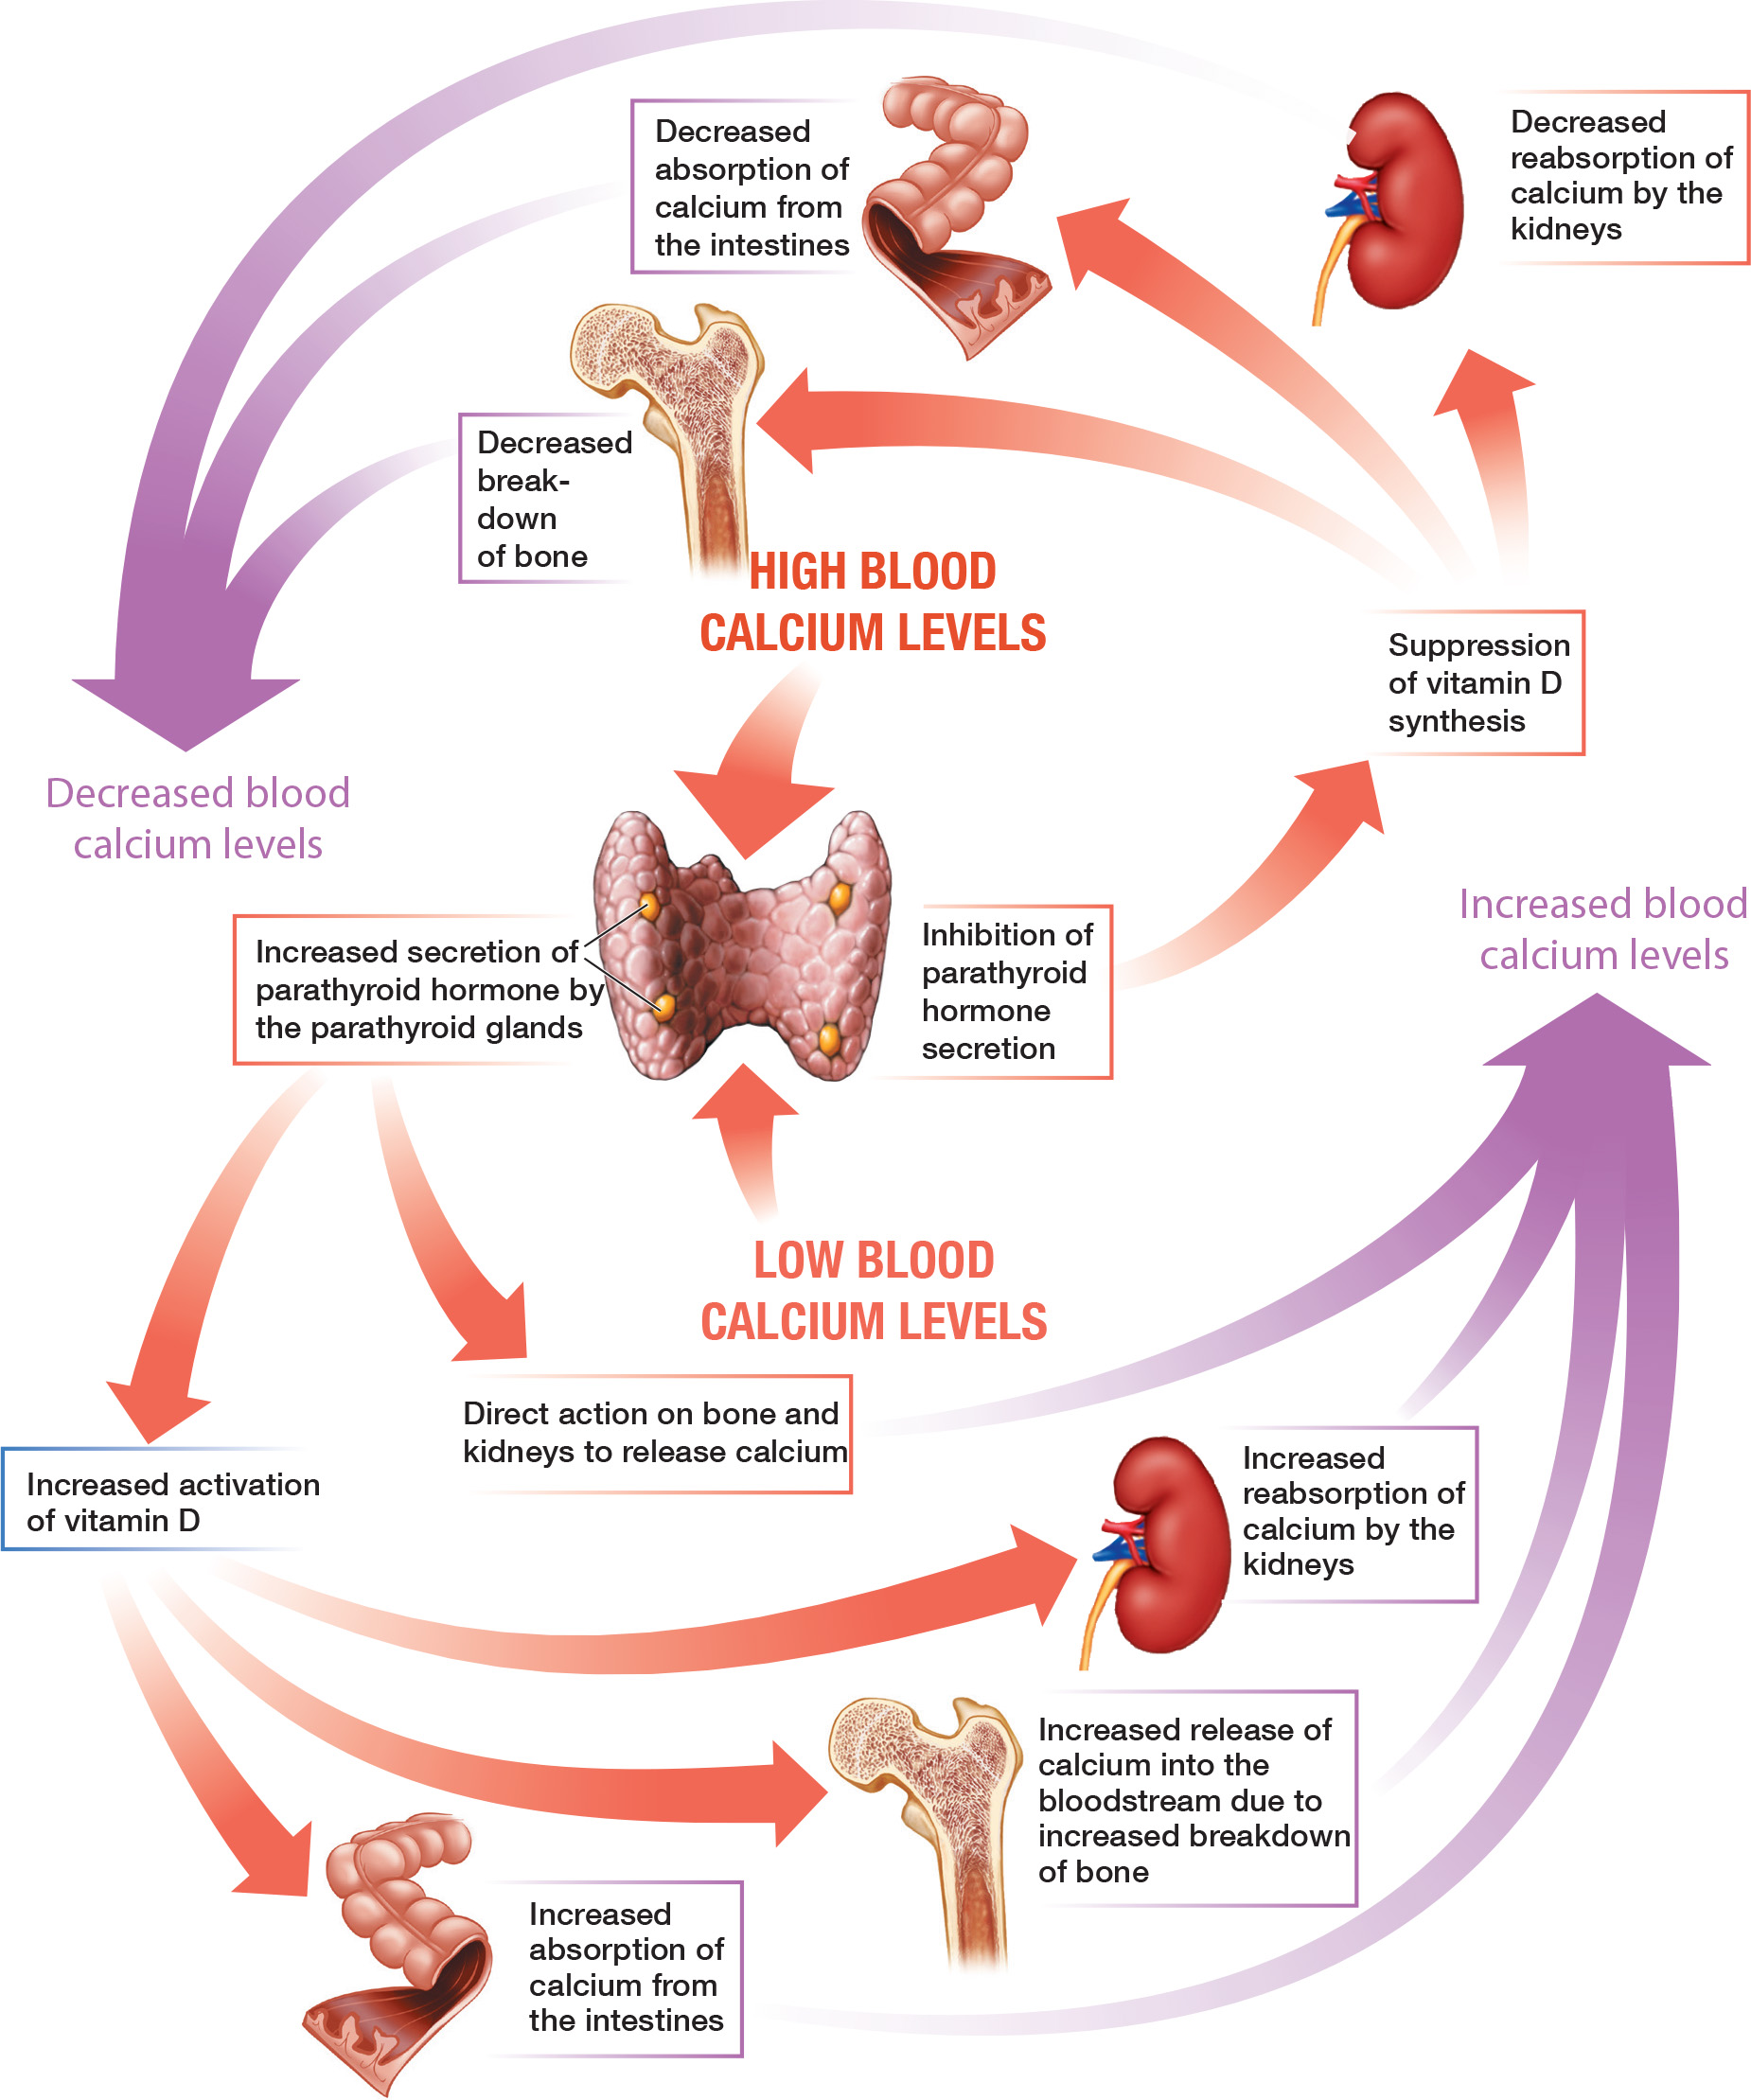
\includegraphics[width=\textwidth]{9_blood-calcium-levels-regulation}
	\caption{Regulation of Blood Calcium Levels}
	\label{fig:regulation-of-blood-calcium-levels}
\end{figure}

\begin{itemize}
	\item Bioavailability: degree to which a nutrient is absorbed
	\item Calcium bioavailability depends on need and age
	\begin{itemize}
		\item Infants, children, and adolescents can absorb more than 60\%
		\item Pregnant and lactating women can absorb 50\%
		\item Healthy adults typically absorb 30\%
		\item Older adults absorb less
		\item Bodies cannot absorb over 500 mg at one time
		\item Numerous factors in food influence absorption
	\end{itemize}
\end{itemize}

\begin{figure}[H]
	\centering
	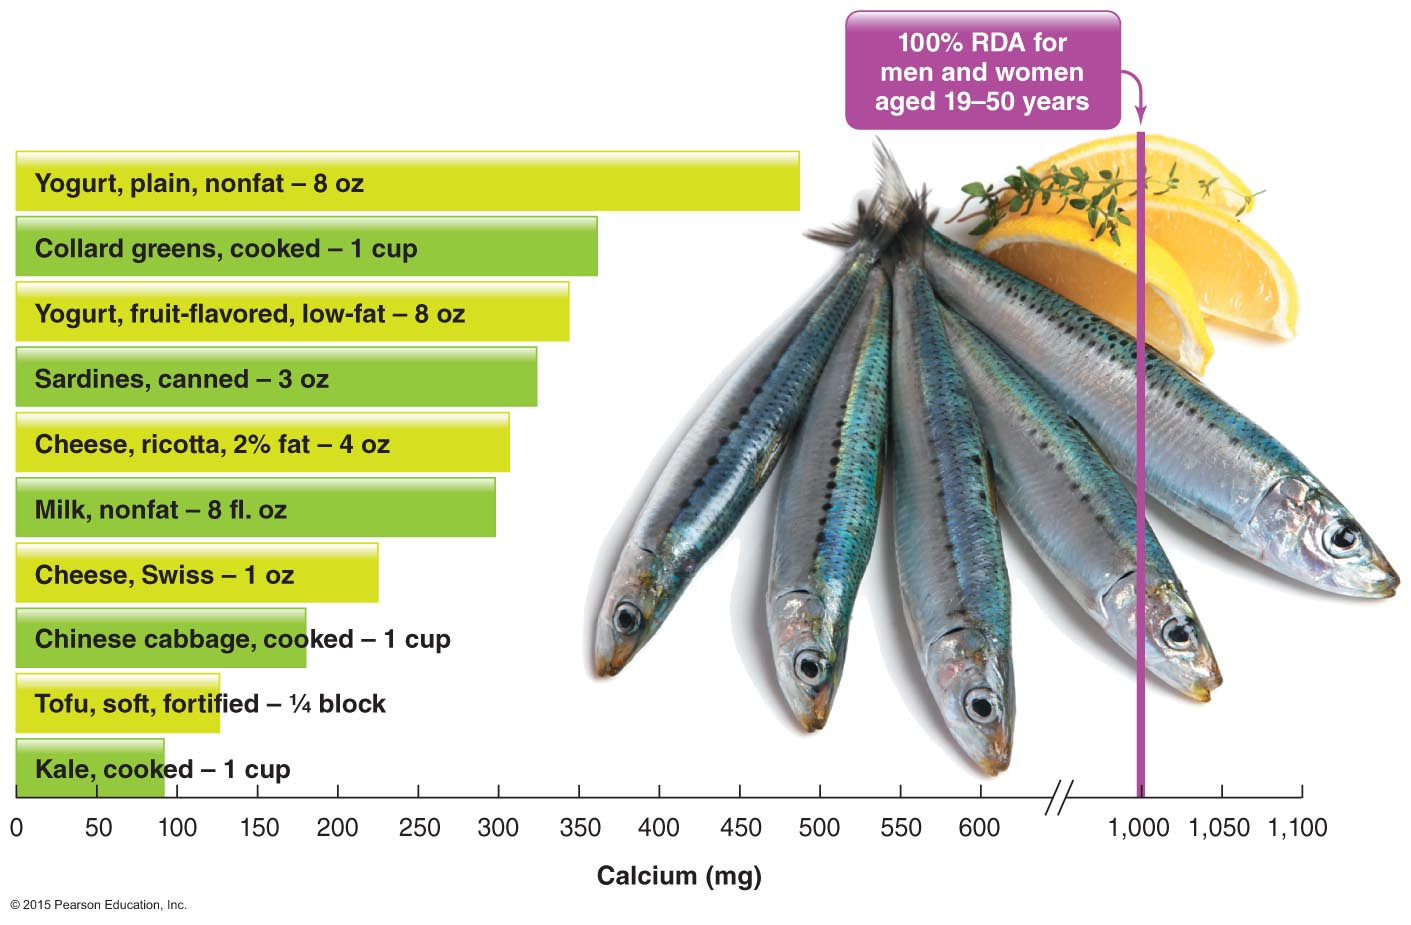
\includegraphics[width=\textwidth]{9_common_sources_calcium}
	\caption{Common Food Sources of Calcium}
	\label{fig:calcium-common-food-sources}
\end{figure}

\begin{itemize}
	\item What if you consume too much calcium?
	\begin{itemize}
		\item Excess calcium is excreted from the body
		\item Calcium supplements can lead to mineral imbalances
		\item Hypercalcemia (high blood calcium) can be caused by cancer and overproduction of PTH
	\end{itemize}
	\item What if you don’t consume enough calcium?
	\begin{itemize}
		\item Hypocalcemia (low blood calcium) can be caused by kidney disease or vitamin D deficiency
	\end{itemize}
\end{itemize}

\section{Phosphorus}\label{sec:Phosphorus}
\begin{itemize}
	\item Phosphorus (as phosphate) is the primary intracellular negatively charged electrolyte
	\item Functions of phosphorus
	\begin{itemize}
		\item Critical to mineral composition of bone
		\item Required for proper fluid balance
		\item Component of lipoproteins, cell membranes, DNA and RNA, and several energy molecules
	\end{itemize}
	\item Recommended intake
	\begin{itemize}
		\item RDA for phosphorus is 700 mg/day
	\end{itemize}
	\item Sources of phosphorus
	\begin{itemize}
		\item High in protein-containing foods such as milk, meats, and eggs
		\item In processed foods as a food additive
		\item In soft drinks as phosphoric acid
	\end{itemize}
	\item What if you consume too much phosphorus?
	\begin{itemize}
		\item Kidney disease and excessive vitamin D supplements or consumption of too many phosphorus-containing antacids can cause elevated phosphorus levels, muscle spasms, and convulsions
	\end{itemize}
	\item What if you don’t consume enough phosphorus?
	\begin{itemize}
		\item Deficiencies are rare in healthy adults
	\end{itemize}
\end{itemize}

\section{Magnesium}\label{sec:Magnesium}
\begin{itemize}
	\item The bones contain 50---60\% of the body’s magnesium
	\item Functions of magnesium
	\begin{itemize}
		\item A mineral found in bone structure
		\item Cofactor for over 300 enzyme systems
		\item Required for the production of ATP
		\item Plays an important role in DNA and protein synthesis and repair
	\end{itemize}
	\item Recommended intake
	\begin{itemize}
		\item RDA varies based on age and gender
		\item 310 mg/day for women aged 19--30
		\item 400 mg/day for men aged 19--30
	\end{itemize}
	\item Sources of magnesium
	\begin{itemize}
		\item Green leafy vegetables, whole grains, seeds, nuts, seafood, beans, some dairy products
	\end{itemize}
\end{itemize}

\begin{figure}[H]
	\centering
	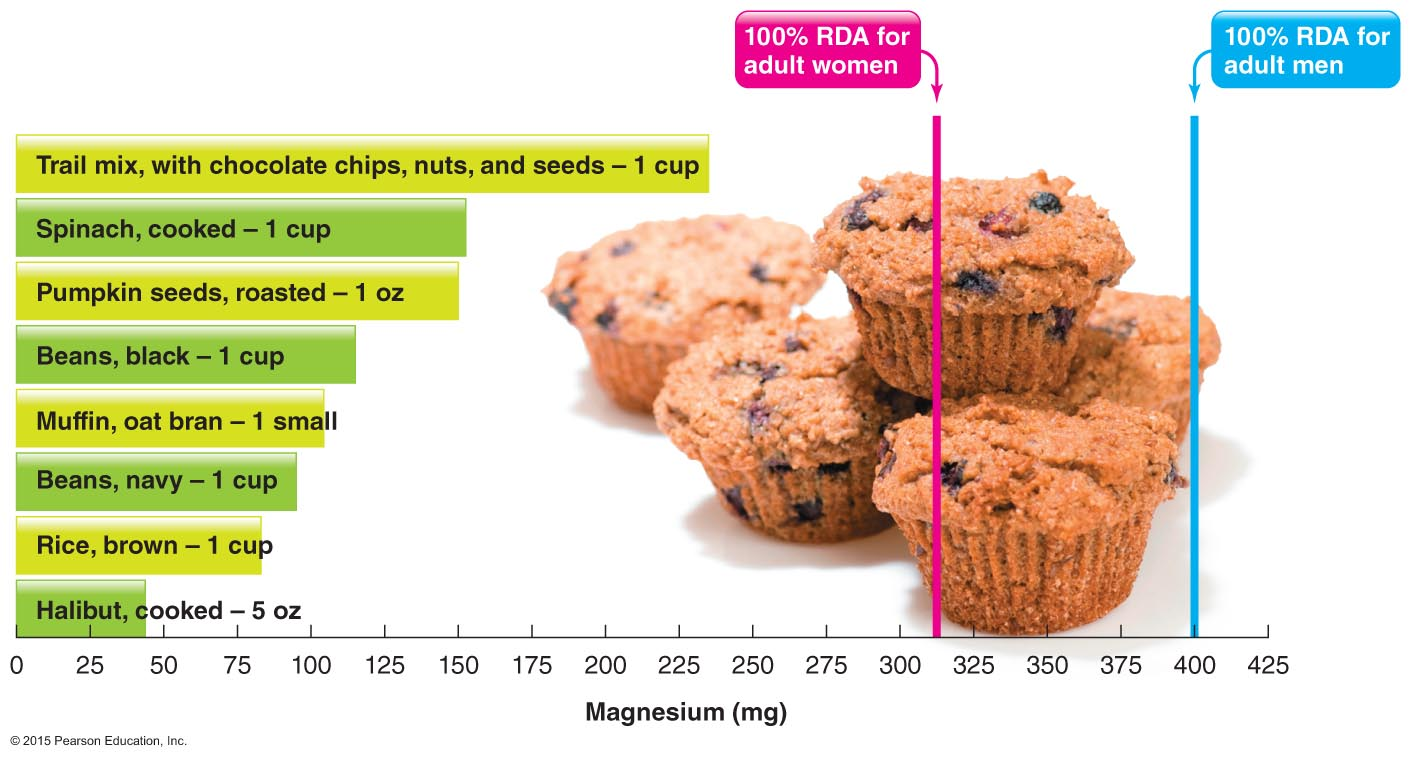
\includegraphics[width=\textwidth]{9_common_sources_magnesium}
	\caption{Common Food Sources of Magnesium}
	\label{fig:magnesium-common-food-sources}
\end{figure}

\begin{itemize}
	\item What if you consume too much magnesium?
	\begin{itemize}
		\item No toxicity from magnesium in food
		\item Magnesium supplements can cause diarrhea, nausea, cramps, dehydration, and cardiac arrest
		\item \definition{Hypermagnesemia}{high blood magnesium levels}
	\end{itemize}
	\item What if you don’t consume enough magnesium?
	\begin{itemize}
		\item Hypomagnesemia can result in low blood calcium and osteoporosis
		\item Other symptoms include muscle cramps, spasms, nausea, weakness, and confusion
	\end{itemize}
\end{itemize}

\section{Fluoride}\label{sec:Fluoride}
\begin{itemize}
	\item Fluoride is a trace mineral
	\begin{itemize}
		\item 99\% of the body’s fluoride is stored in teeth and bones
	\end{itemize}
	\item Functions of fluoride
	\begin{itemize}
		\item Development and maintenance of teeth and bones
		\item Combines with calcium and phosphorus to make tooth enamel stronger, which protects teeth from dental caries (cavities)
	\end{itemize}
	\item Recommended intake
	\begin{itemize}
		\item RDA for women is 3 mg/day
		\item RDA for men is 4 mg/day
	\end{itemize}
	\item Sources of fluoride
	\begin{itemize}
		\item Fluoridated dental products
		\item Fluoridated water
	\end{itemize}
	\item What if you consume too much fluoride?
	\begin{itemize}
		\item \definition{Fluorosis (excess fluoride)}{creates porous tooth enamel; teeth become stained and pitted}
	\end{itemize}
	\item What if you don’t consume enough fluoride?
	\begin{itemize}
		\item Dental caries (cavities)
	\end{itemize}
\end{itemize}

\begin{figure}[H]
	\centering
	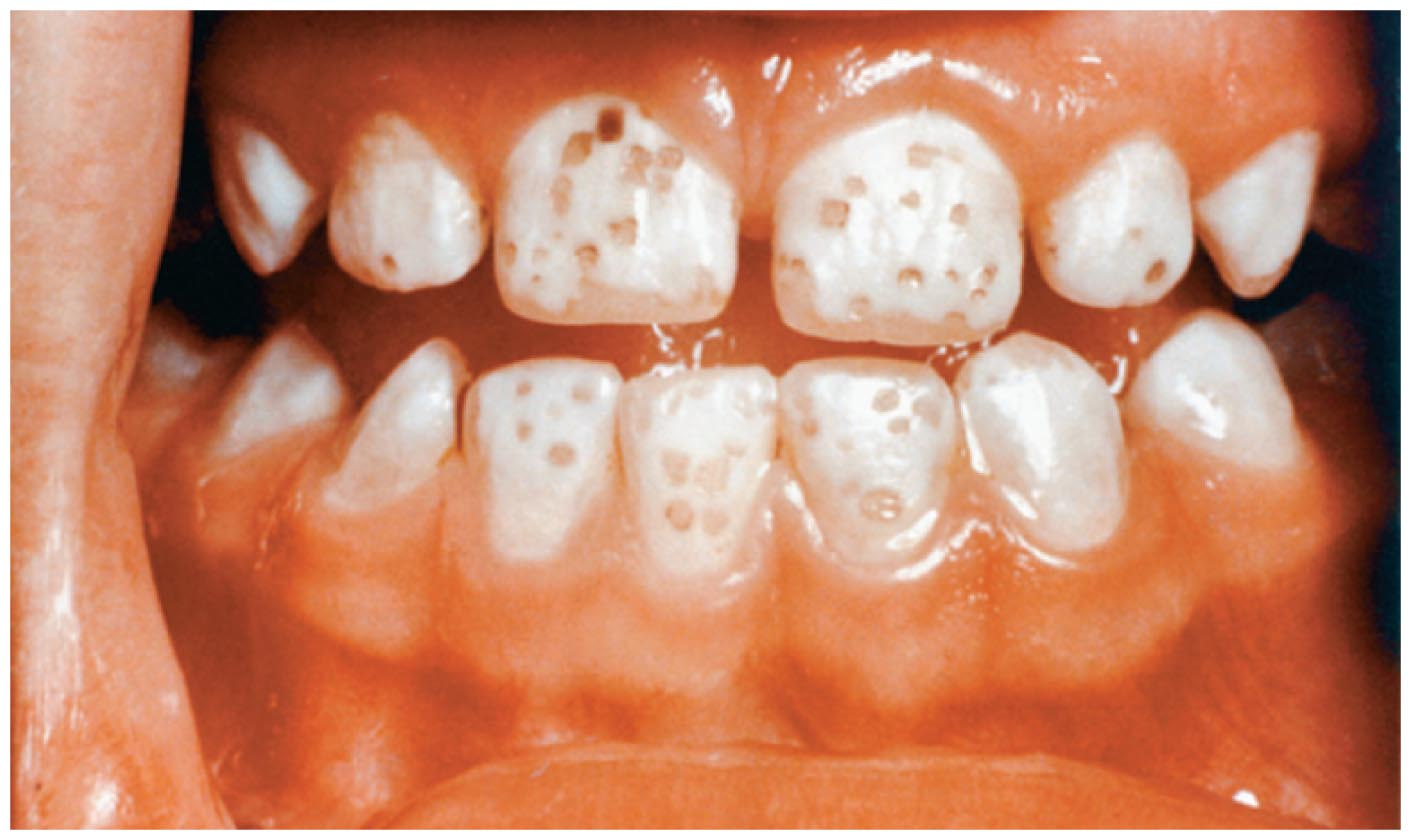
\includegraphics[width=\textwidth]{9_fluorosis}
	\caption{Fluorosis}
	\label{fig:fluorosis}
\end{figure}

\section{Vitamin D}\label{sec:Vitamin D}
\begin{itemize}
	\item Fat-soluble vitamin
	\item Excess is stored in liver and fat tissue
	\item Can be synthesized by the body by exposure to UV light from the sun
	\item Is considered a hormone because it is synthesized in one location and acts in other locations
\end{itemize}

\begin{figure}[H]
	\centering
	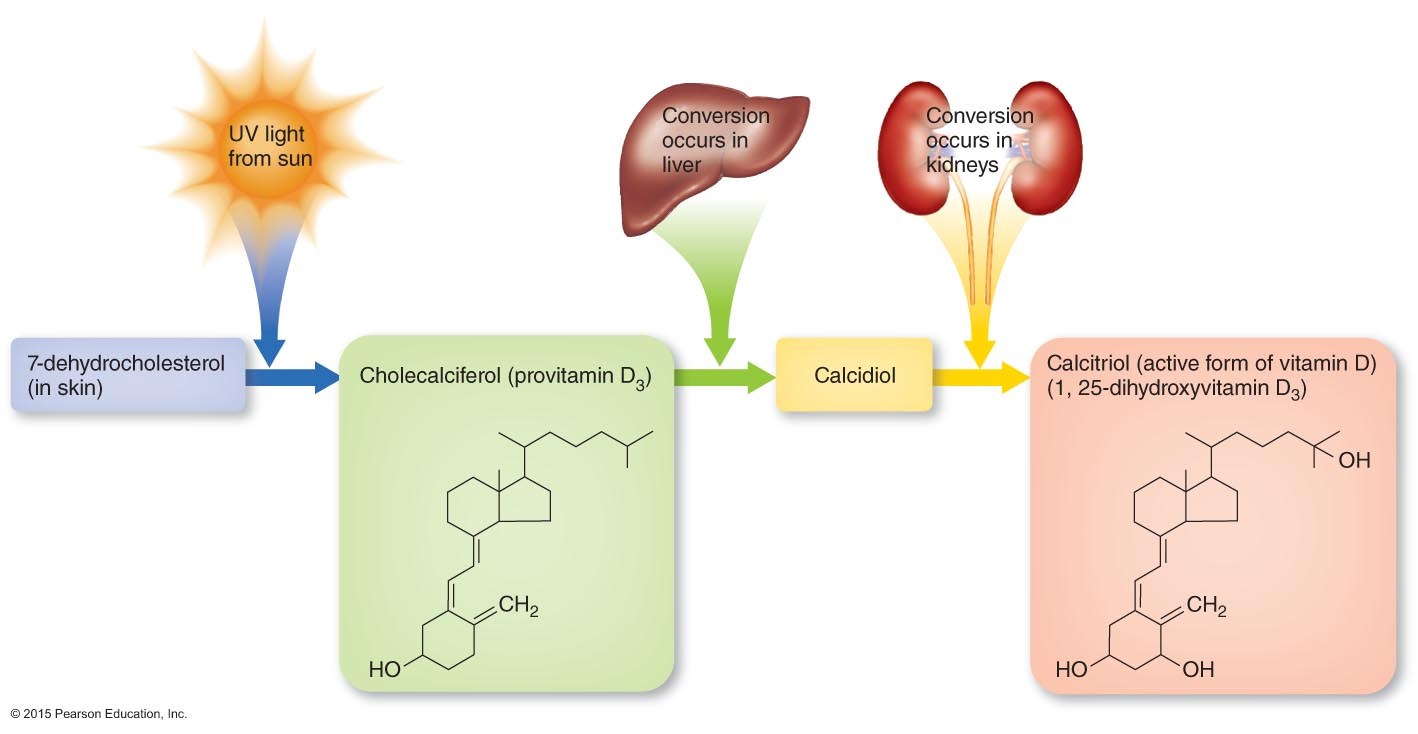
\includegraphics[width=\textwidth]{9_vitamin_d_sunlight}
	\caption{Conversion of Sunlight into Vitamin D}
	\label{fig:conversion-of-sunlight-into-vitamin-d}
\end{figure}

\begin{figure}[H]
	\centering
	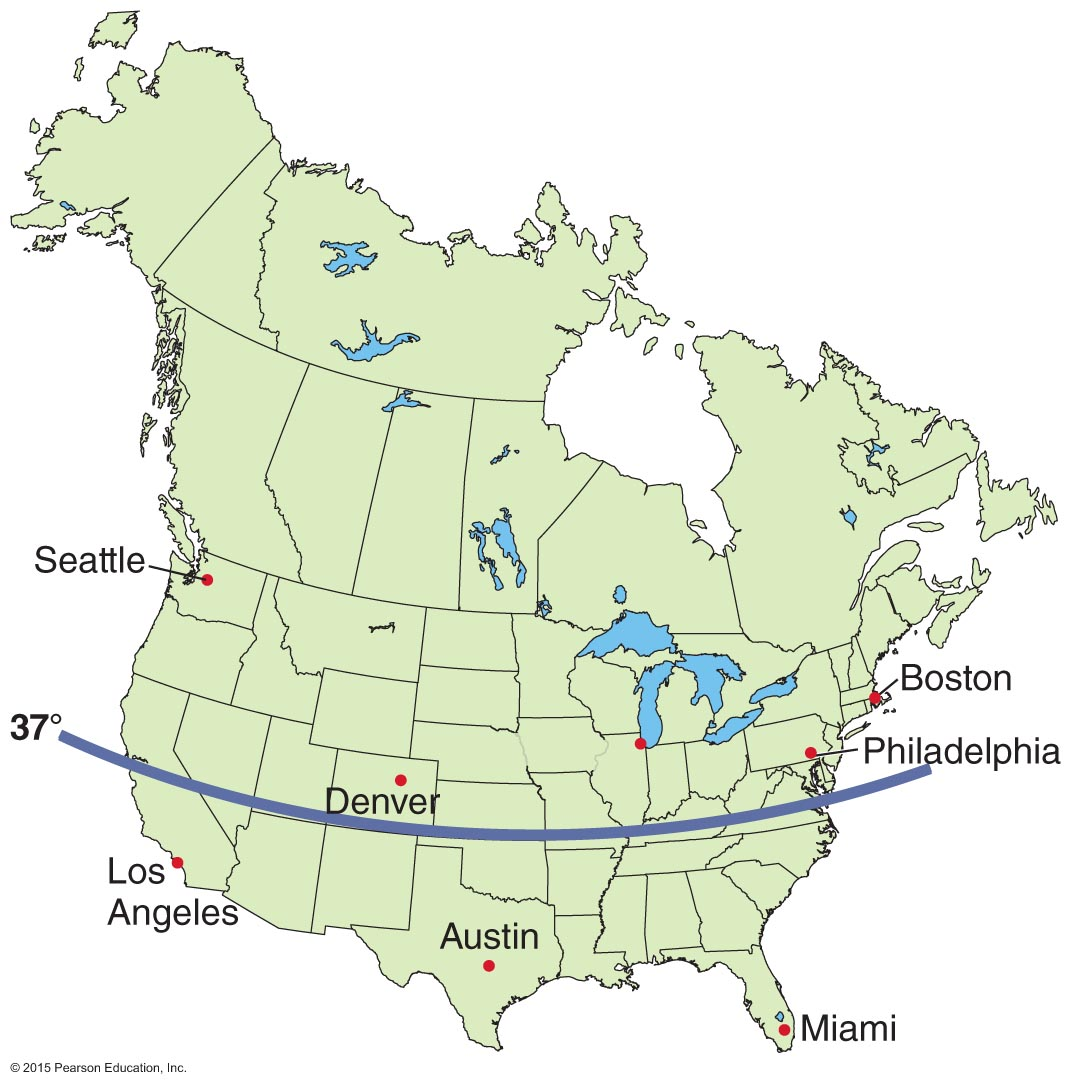
\includegraphics[width=\textwidth]{9_vitamin_d_sunlight_north_america}
	\caption{Vitamin D and Sunlight in North America}
	\label{fig:vitamin-d-sunlight-north-america}
\end{figure}

\begin{itemize}
	\item Functions of vitamin D
	\begin{itemize}
		\item Required for calcium and phosphorus absorption
		\item Regulates blood calcium levels
		\item Stimulates osteoclasts
		\item Necessary for calcification of bone
	\end{itemize}
	\item Sources of vitamin D
	\begin{itemize}
		\item Most foods naturally contain very little vitamin D
		\begin{itemize}
			\item Vitamin $\mbox{D}_{2}$ or ergocalciferol is found in plant foods
			\item Vitamin $\mbox{D}_{3}$ or cholecalciferol is found in animal foods
		\end{itemize}
	\end{itemize}
	\item Most vitamin D is obtained from fortified foods such as milk and cereal products
	\item Vegetarians not consuming dairy foods receive vitamin D from the sun, fortified soy products, or supplements
\end{itemize}

\begin{figure}[H]
	\centering
	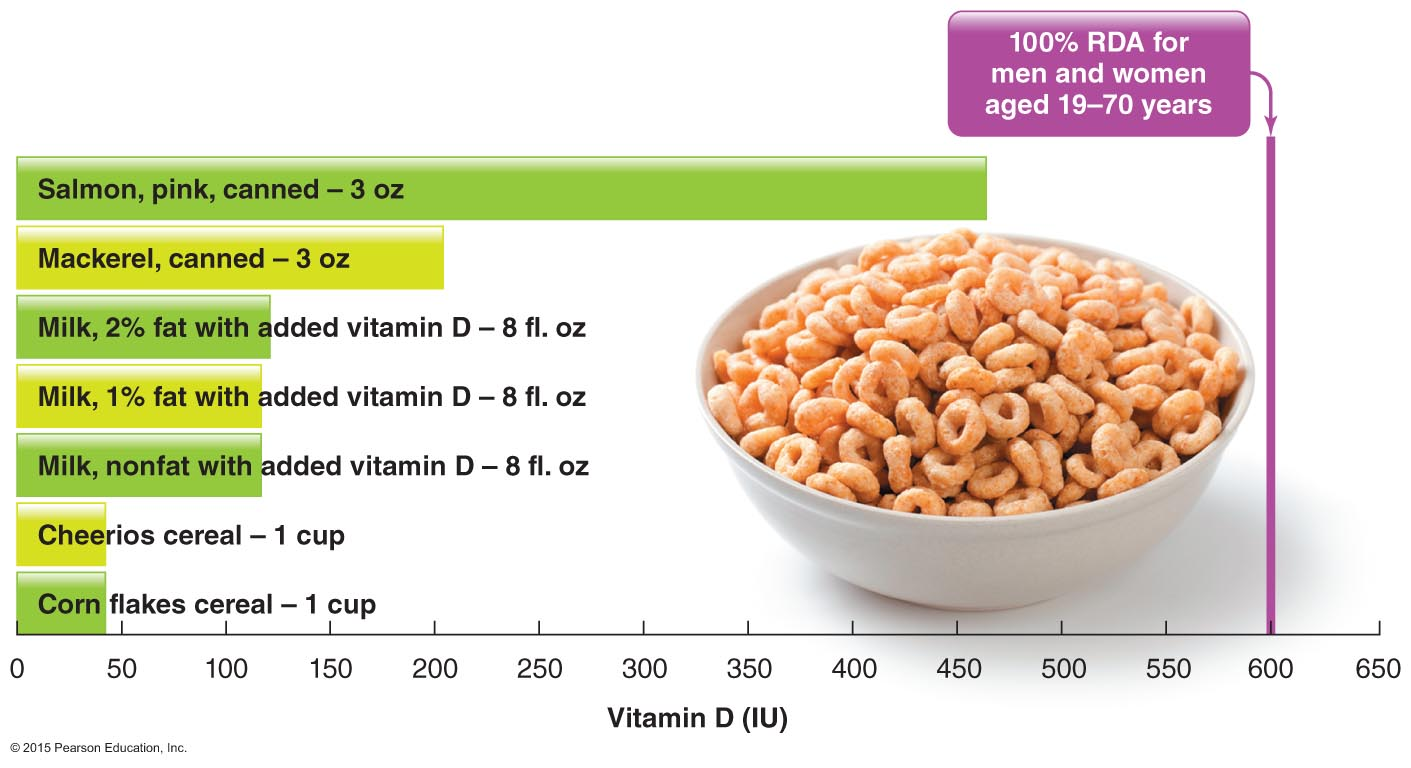
\includegraphics[width=\textwidth]{9_common_sources_vitamin_d}
	\caption{Common Food Sources of Vitamin D}
	\label{fig:common-sources-vitamin-d}
\end{figure}

\begin{itemize}
	\item What if you consume too much vitamin D?
	\begin{itemize}
		\item Occurs with vitamin supplements, not excessive exposure to sunlight
		\item Results in \definition{hypercalcemia}{high blood calcium}
	\end{itemize}
	\item What if you don’t consume enough vitamin D?
	\begin{itemize}
		\item Occurs with diseases that reduce intestinal absorption of fat and limited exposure to sunlight
		\item \definition{Rickets}{inadequate mineralization or demineralization of bones}; occurs in children
		\item \definition{Osteomalacia}{loss of bone mass in adults}
	\end{itemize}
\end{itemize}

%\begin{figure}[H]
%	\centering
%	\includegraphics[height=0.75\textwidth]{9_rickets}
%	\caption{Rickets}
%	\label{fig:rickets}
%\end{figure}

\section{In Depth: Osteoporosis}\label{sec:in-depth:-osteoporosis}
\begin{itemize}
	\item Osteoporosis is a disease characterized by
	\begin{itemize}
		\item Low bone mass
		\item Deterioration of bone tissue
		\item Fragile bones, leading to bone fractures
		\item Compaction of bone; decreased height
		\item Shortening and hunching of the spine: dowager’s hump
	\end{itemize}
\end{itemize}

\begin{figure}[H]
	\centering
	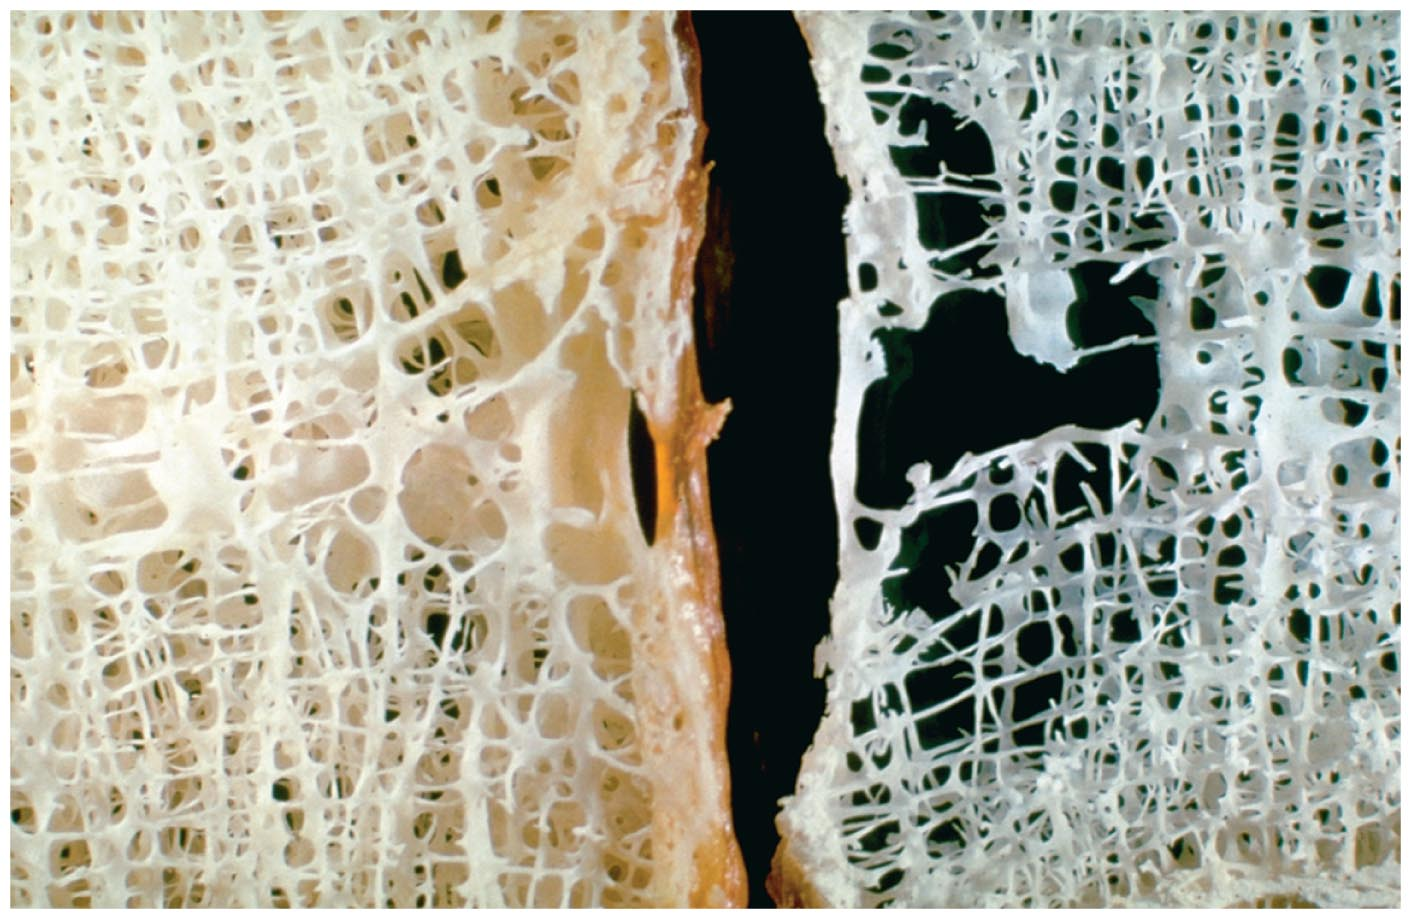
\includegraphics[width=\textwidth]{9_osteoporosis}
	\caption{Osteoporosis}
	\label{fig:osteoporosis}
\end{figure}

\begin{figure}[H]
	\centering
	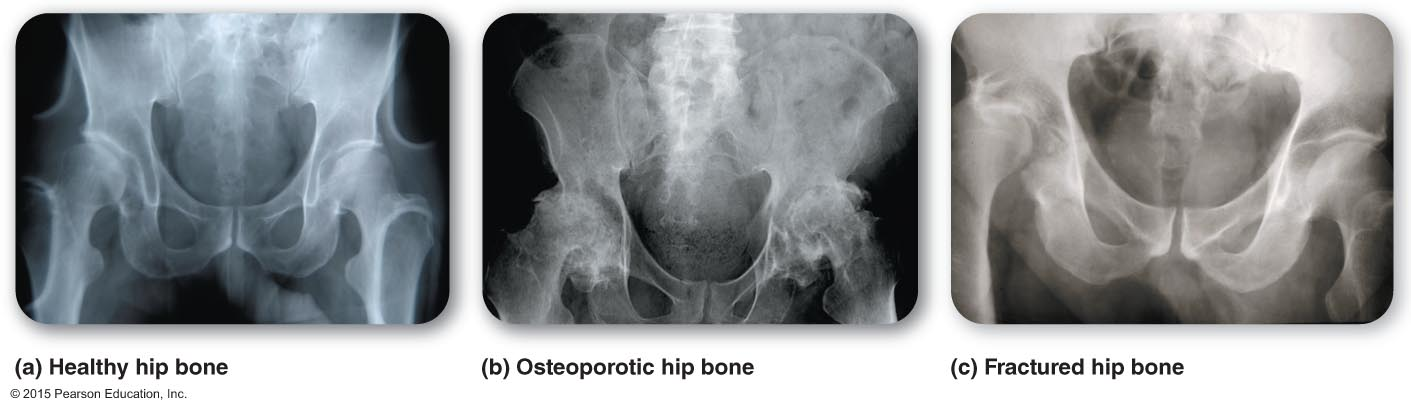
\includegraphics[width=\textwidth]{9_osteoporosis_hips}
	\caption{Osteoporosis}
	\label{fig:osteoporosis-hips}
\end{figure}

\begin{itemize}
	\item Factors influencing the risk of osteoporosis include
	\begin{itemize}
		\item Age
		\item Gender
		\item Genetics
		\item Tobacco, alcohol, and caffeine use
		\item Nutrition
		\item Physical activity
		\item History of amenorrhea (loss of menstrual function)
	\end{itemize}
\end{itemize}

\begin{table}[H]
	\centering
	\begin{threeparttable}
		\caption{Risk Factors for Osteoporosis}
		\label{tab:risk-factors-for-osteoporosis}
		\rowcolors{2}{rowmedgreen}{rowlightgreen}
		\begin{tabular}{p{0.5\textwidth} p{0.5\textwidth}}
			\rowcolor{rowdarkgreen}\textbf{Modifiable Risk Factors} & \textbf{Nonmodifiable Risk Factors}\\
			Smoking & Older age (elderly)\\
			Low body weight & Caucasian or Asian race\\
			Low calcium intake & History of fractures as an adult\\
			Low sun exposure & Family history of osteoporosis\\
			Alcohol abuse & Gender (female)\\
			History of amenorrhea (failure to menstruate) in women with inadequate nutrition & History of amenorrhea (failure to menstruate) in women with no recognizable cause\\
			Estrogen deficiency (females) & \\
			Testosterone deficiency (males) & \\
			Repeated falls & \\
			Sedentary lifestyle & \\
			\rowcolor{rowdarkgreen} & \\
		\end{tabular}
		\begin{tablenotes}
			\small
			\item Source: Information adapted from the National Osteoporosis Society. 2014. Factors that increase your risk of osteoporosis and fracture. \url{https://www .nos.org.uk/healthy-bones-and-risks/are-you-at-risk}
		\end{tablenotes}
	\end{threeparttable}
\end{table}

\begin{itemize}
	\item Age is a factor for osteoporosis because
	\begin{itemize}
		\item Bone mass decreases with age
		\item Age-related hormonal changes influence bone density (reduced estrogen and testosterone production)
		\item Older adults are less able to absorb vitamin D
	\end{itemize}
	\item Gender is a risk factor for osteoporosis
	\begin{itemize}
		\item 80\% of Americans with osteoporosis are women
		\item Women have lower bone density than men
		\item Estrogen loss in postmenopausal women causes increased bone loss
		\item Women live longer than men
		\item Social pressure on girls to be thin leads some to harmful dieting when bone mass is still building
	\end{itemize}
\end{itemize}

\begin{figure}[H]
	\centering
	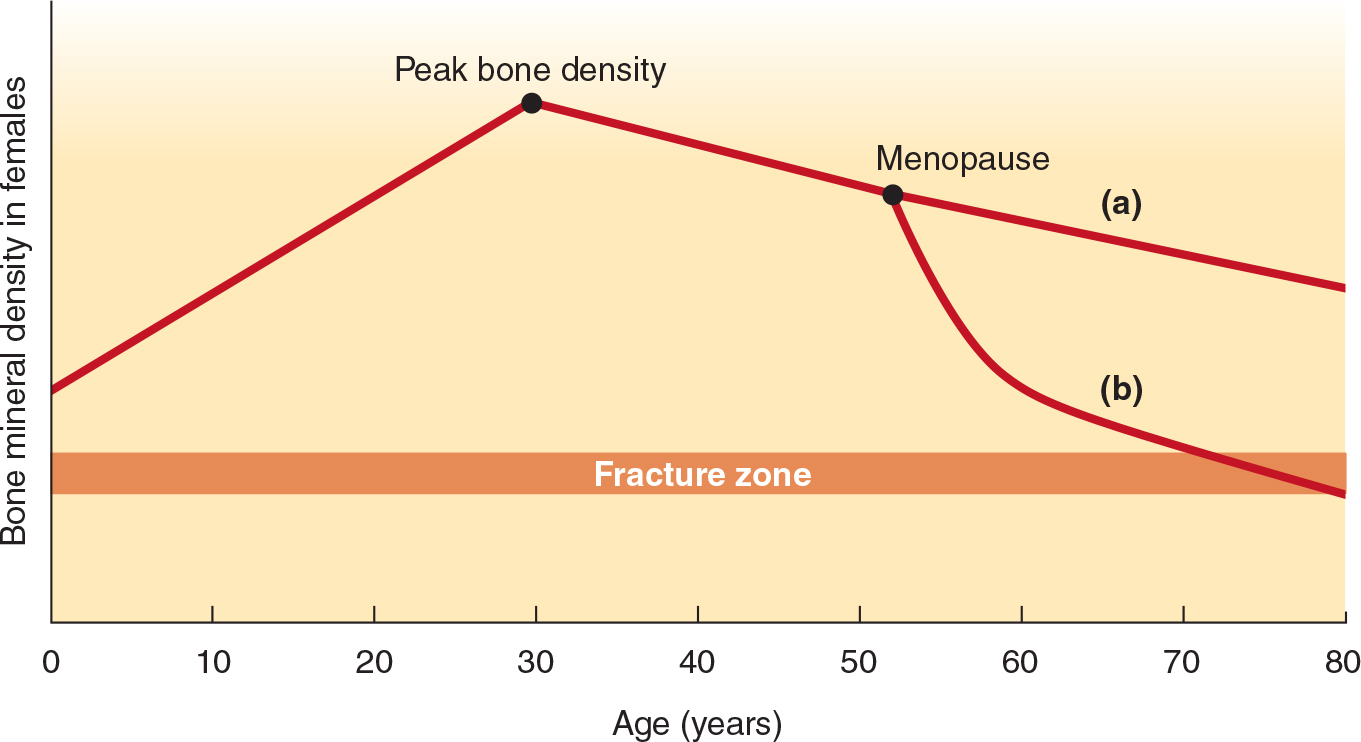
\includegraphics[width=\textwidth]{9_osteoporosis_age}
	\caption{Osteoporosis}
	\label{fig:osteoporosis-age}
\end{figure}

\begin{itemize}
	\item Tobacco, alcohol, and caffeine use
	\begin{itemize}
		\item Cigarette smoking decreases bone density due to its effects on hormones that influence bone formation and resorption
	\end{itemize}
	\item Alcohol consumption beyond 1--2 drinks per day is associated with a higher risk of fractures
	\item Caffeine increases calcium loss in the urine
	\item Nutritional factors influence risk
	\begin{itemize}
		\item Diets high in fruits and vegetables are associated with improved bone health
	\end{itemize}
	\begin{itemize}
		\item Physical activity influences risk
	\end{itemize}
	\begin{itemize}
		\item Regular exercise causes stress to bones, leading to increased bone mass
		\item Weight-bearing activities (walking, jogging) are especially helpful in increasing bone mass
	\end{itemize}
	\item There is no cure for osteoporosis
	\item The progression of osteoporosis may be slowed by
	\begin{itemize}
		\item Adequate calcium and vitamin D intake
		\item Regular exercise
		\item Some medications, including hormone replacement therapy (HRT)
	\end{itemize}
\end{itemize}

\end{document}
